\documentclass[12pt,fleqn]{report}
\usepackage[utf8]{inputenc}
\usepackage{amssymb,amsmath}
\usepackage{times}                     % times new roman
\usepackage{listings}
\usepackage{textcomp}                   % listings environment
\usepackage{braket}
\usepackage{latexsym}
\usepackage{setspace}
\usepackage{hyperref}
\usepackage{graphicx}
\usepackage{enumitem}                  % to start itemization an optional number
\usepackage{color}
\usepackage{floatrow}
\floatsetup[table]{capposition=top}     % to take caption to top for tables
\usepackage[left=4.0cm, top=2.5cm, bottom=2.5cm, right=2.5cm]{geometry}
%\title{Application of the Density Matrix Renormalization Group Method to the Single Particle Problem}
%\author{Nur Aslan}
\usepackage{amsthm}

\begin{document}

\thispagestyle{empty}
\pagestyle{empty}
%\begin{figure}
%\begin{center}
%\raggedright
\hspace{-1.8cm}
%\includegraphics[scale=0.8]{./title}
%\end{center}
%\newgeometry{left=2.5cm}
%\end{figure}

\newpage

%\restoregeometry
\pagenumbering{roman}
\onehalfspacing
\pagestyle{plain}
\tableofcontents
\newpage
\author{Onur Kaplan}
\begin{abstract}
\thispagestyle{plain}
\pagenumbering{roman}
\setcounter{page}{3}
\addcontentsline{toc}{chapter}{Abstract}
	
In this project, we studied the Monte Carlo method to calculate statistical properties of a classical system because of its pedagogical popularity, instructional value and physical importance. We carried out Monte Carlo simulations for Ising Model in 2D. We have considered two algorithms to simulate Ising Model, they are Metropolis algorithm and Wolff algorithm and we compared these two algorithms. After studying and demonstrating the Metropolis algorithm, we discuss the so called "critical slowing down" problem towards the critical temperature. A solution to this problem is given by the Wolff algorithm which is discussed at the end. 

\end{abstract}


%\newpage
\thispagestyle{plain}
\pagenumbering{roman}
\setcounter{page}{5}
\addcontentsline{toc}{chapter}{List of Figures}
\listoffigures


\chapter{Introduction}
\pagenumbering{arabic}

\section{History of Monte Carlo Method}

In 1945's a team which is adminstrated by John Mauchly and Presper Eckert was working on the first computer, ENIAC at University of Pensylvania. Also, John von Neumann and Edward Teller were interested in thermonuclear problem at Los Alamos. When ENIAC was almost completed, Neumann decided to set a model for a thermonuclear reaction to test the ENIAC and to realize it, he asked Stan Frankel and Nicholas Metropolis to work with him. Then, after getting some information about the ENIAC, they started to work for the model at Los Alamos. However, because of the World War during this time period, they could not finish their work. After that, Stanislaw Ulam joined the laboratory at Los Alamos. 
Ulam's extensive mathematical background made him aware that statistical sampling techniques had fallen into desuetude because of the length and tediousness of the calculations.\cite{mc}  At the laboratory, he recognized the first electronic computer ENIAC and he was impressed by the speed of ENIAC. Ulam was interested in branching process and Neutron multiplication in fission device and Ulam wanted to solve Neutron diffusion, statistically by using ENIAC. At that time, Metropolis suggested an obsious name for the statistical method - a suggestion not unrelated to the fact that Ulam had an uncle who would borrow money from relatives because he "just had to go to Monte Carlo". \cite{mc}.

\section{Random Numbers for Monte Carlo Simulation}


Monte Carlo method is a statistical approach to physical processes. To realize Monte Carlo method in any computer, random sampling and random decisions should be encountered. Hence, we want to get random numbers from a computer.

Actually, firstly we should ask that how can we get a random number in nature?  To get a randomness from the nature, we have to analyze probabilistic nature of Quantum Mechanics. According to the Quantum Mechanics, for an unstable nuclei, when the radioactive decay will occur, is random. Hence, if we save the times that decaying occurs, we get truly random numbers. Thus, using radioactive decay, we may create random numbers for our simulation. Also, in the computers, people generate these random numbers, called pseudo-random numbers, with respect to an algorithm; therefore, numbers are predetermined. We expect that these numbers created by algorithm to have an uniform distribution, to be in a definite range and to have minimum correlation. These correlations in the numbers means that actually, we don't create numbers that are completely random. Thus, we label them as 'pseudo-random' numbers. Hence, this lack of randomness effect the Monte Carlo simulation and causes an error in the simulation. 
 
Suppose we want to create pseudo-random integer numbers($k_n$) between 0 and L. Most widely used algorithm for that is $k_n = f(k_{(n-1)})$, f is a function that returns integers. The number that is generated is dependent on the previous number. To generate pseudo-random integer we need a 'seed' to start the algorithm. After, we input a seed, the algorithm continuously creates pseudo-random numbers. However, if we get a number that was created before, we enter a cycle, and we get same numbers, periodically. Hence, we want that the cycle to be very long because when we are creating pseudo-random numbers, we should not enter the cycle twice. For a more complex algorithm, $k_n = f(k_{(n-1)}, k_{(n-2)}, ...)$ can be used. With using transformations on created numbers, we can arrange the range in which numbers are generated.

Because an algorithm is used to create numbers are determined, hence, these numbers are deterministic, not random. If we enter same seeds to the algorithm we get same numbers. Thus, there is no randomness in the algorithm for a given seed. Numbers that are generated only obey the rules of algorithm and mathematics. And if true randomness cannot be created in any mathematical operation, then it will have to come from some physical process. \cite{random}


 \section{Monte Carlo Method}

In the most general terms, Monte Carlo method is a statistical - almost experimental - approach to computing integrals using random positions, called samples, whose distribution is carefully chosen. \cite[p. 1]{krauth}

In Monte Carlo simulations two basic sampling methods exist; 

One of them is direct sampling. 
Assume that we are in a 1D space which has sites. 
In the direct sampling method, we take samples independently for each step with choosing a random site on the space. Hence, if we use real random numbers, our new samples are independent of the previous ones, because we choose a new site randomly. With taking samples again and again, we sweep out the space and by using these samples, we can make calculations. Other sampling method is Markov-Chain sampling. In the Markov-Chain sampling, our sample depends on the previous sample. Firstly, we start sampling from an initial site that is given or where the last simulation ends.  Then, from the initial site, we move to another site on the space, in any direction and distance. This direction and distance again random, but, distance is limited to a value $\delta$. With using this procedure, we visit other states and if the resulting state is a state that we don't want to be in there, then we reject the move. Hence, this limitation for the moves $\delta$ affects the rejection rate. If $\delta$ is very large, rejection rate is so high, this means that we generally don't move to another state; thus, our traveled path is small. Also, if $\delta$ is very small, acceptance rate is so high, this means that we generally move from state to another state; however, in this case our $\delta$ is small; therefore , our traveled path is, again, small. Thus, when $\delta$ is on the edge , very large or small, we can't sweep out most of the states and calculation of the integral by samples may fail. 

Instead of calculating the integral analitically, we are taking samples and using these samples we approximate the integrals in discrete manner. Thus, Monte Carlo method allows the evaluation of high dimensional integrals, such as appearing in statistical physics and other domains, if only we can think of how to generate the samples. \cite[p. 8]{krauth}

Direct sampling is practically impossible for large configuration spaces, hence if we want to sample for large spaces, we must use Markov-Chain sampling. 
	
\section{Basic Implementations of the Monte Carlo Method}

To understand the basic structure of the Monte Carlo method, we will illustrate 2 basic examples to calculate $\pi$. To calculate it, we take random samples from inside a square and we count the samples that are inside the circle which is surrounded by the square. In these examples, we used direct sampling and Markov-Chain sampling methods.  

In the first example, we have a square in the range 0 and 1 and we have a one fourth circle inside it, which has a center at origin and radius 1. If we take the ratio of samples that are inside of the circle (hits) to all samples, we expect that this ratio is $ r= \frac{\pi r^2}{4}$  . In this example, we used direct sampling method to take samples. We take N=1000,10000, ... , $10^7$ samples, respectively and we calculated the ratio of hits to all samples. And we estimate the mean square deviation. If we plot mean square deviation, $E[(\frac{Nhits}{N} - \frac{\pi}{4})^2]$, with respect to N, we get,

\begin{figure}[ht!]
\centering
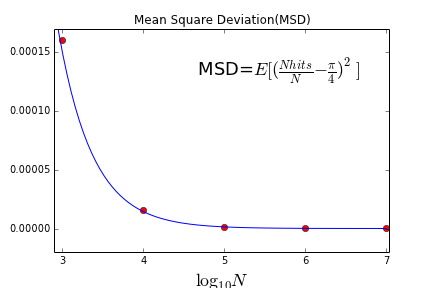
\includegraphics[width=110mm]{../programs/MC/Pi/mean_square_deviation_direct_sampling.png}
\caption{Mean Square Deviation for N = 1000,10000,... , respectively}
\end{figure}
Hence, with direct sampling method, we can calculate $\pi$ with high precision for a small space. 

In the second example, we have a square centered at origin and length 2 and we have a circle inside it which has a center at origin and radius 1. Again, we expect that the ratio to be $r= \frac{\pi}{4}$. However, in this case we used Markov-Chain sampling instead of direct sampling. In this case we take N=$4*10^6$ samples. If we look at Mean square deviation, 
\begin{figure}[ht!]
\centering
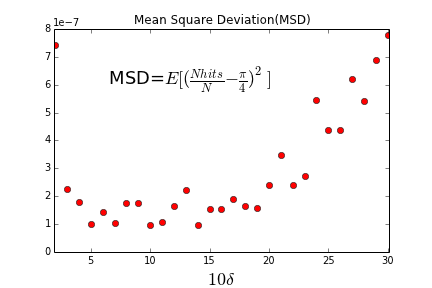
\includegraphics[width=110mm]{../programs/MC/Pi/mean_square_deviation_Markov_sampling.png}
\caption{Mean Square Deviation for $\delta$= 0.2,0.3,...,3.0 , respectively}
\end{figure}
We can see that when $\delta$ is 0.8 we get maximum precision. 

If we look at rejection rate, 

\begin{figure}[ht!]
\centering
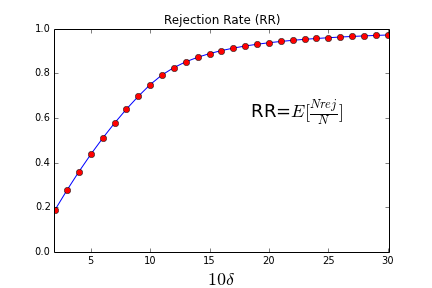
\includegraphics[width=120mm]{../programs/MC/Pi/rejection_rate_Markov_sampling.png}
\caption{Rejection rate for $\delta$= 0.2,0.3,...,3.0 , respectively}
\end{figure}
when $\delta$ is 0.8, we have a rejection rate is around $0.55$.

\section{Gaussian Distribution and Central Limit Theorem}

\subsection{Gaussian Distribution}

In various situations, histograms of measurements looks like a bell shaped curve. This bell shaped curve is known as \textit{Gaussian Distribution}. Gaussian distribution, which appears in a lot of practical applications, is a continuous probability distribution. Because Gaussian random variables arise in so many practical situations, statisticians refer to them as normal random variables.\cite[p. 248]{wiley}.  
\newtheorem*{gauss*}{Gaussian Distribution}
\begin{gauss*}
If X is an Gaussian Random Variable, the Probability Distribution Function (PDF) of X is
$$f_X(x) = \frac{1}{\sqrt{2\pi\sigma^2}}e^\frac{-(x-\mu)^2}{2\sigma^2} $$
where $\mu$  and $\sigma$  are the parameters.
\end{gauss*}
  
The parameter $\mu_x$ is the \textit{Mean Value} or \textit{Expected Value} of the distribution and $\sigma_X$ is the \textit{Standart Deviation} of the distribution and also ${\sigma_x}^2$ is the \textit{Variance}.
For a continuous probability distribution,

\begin{gather}
E[X] = \mu_x = \int_{-\infty}^\infty xf_X(x) \,dx  \\
Var[X] = E[(X-\mu_x)^2] = E[X^2] - {\mu_x}^2
\end{gather}
Also there are 3 useful formulas for mean value and variance where $a,b \in\mathbb{R}$ 
\begin{gather}
E[aX+b] = aE[X] + b  \\
Var[X+b] = Var[X]  \\
Var[aX] = a^2Var[X] 
\end{gather}
which can be easily proven.

When X and Y are 2 random variables
\begin{gather}
Cov[X,Y] = E[(X-\mu_x)(Y-\mu_y)] = E[XY] -\mu_x \mu_y \\
E[X + Y] = E[X] + E[Y] \\
Var[X + Y] = Var[X] + Var[Y] + 2Cov[X,Y]
\end{gather}
again, they can be proven, directly.

\newtheorem*{independence}{Independence of two Random Variables}
\begin{independence}
Random variables X and Y are independent if and only if 
$$ f_{X,Y}(x,y) = f_X(x)f_Y(y)$$
\end{independence}
Hence, when X and Y are 2 independent random variables $Cov[X,Y]=0$

\subsection{Central Limit Theorem (CLT)}
Central Limit Theorem (CLT) explains why so many practical phenomena produce data that can be modeled as Gaussian random variables. CLT is used to calculate probabilities associated with the independent and identically distributed (i.i.d.) sum $$ W_n = X_1 + ... + X_n $$
In this case, $ E[W_n] = n\mu_x $ and $ Var[W_n] = nVar[X] = n {\sigma_x}^2$. As \textit{n} approaches infinity, $ E[W_n]$ and $ Var[W_n] $ approach infinity, so there is no convergence in $E[W_n] $ and $ Var[W_n] $. Therefore, to get rid of this divergence CLT will be explained in terms of standardized random variable 
\newtheorem*{standartrv}{Standardized Random Variable}
\begin{standartrv}
$$ Z_n = \sum\limits_{i=1}^n \frac{X_i - n\mu_x}{\sqrt{n{\sigma_x}^2}} 
 =\frac{W_n - n\mu_x}{\sqrt{n{\sigma_x}^2}}
$$
\end{standartrv}
For standardized random variable $ Z_n $, using above quantities
\begin{equation}
  E[Z_n] =E\left[ \sum\limits_{i=1}^n \frac{X_i - n\mu_x}{\sqrt{n{\sigma_x}^2}}\right] = 
  \frac{E\left[\sum\limits_{i=1}^n X_i\right] - n\mu_x}{\sqrt{n{\sigma_x}^2}} = \frac{E[W_n] -n\mu_x}{\sqrt{n{\sigma_x}^2}} = 0
\end{equation}
\begin{equation}
 Var[Z_n] = Var\left[\sum\limits_{i=1}^n \frac{X_i - n\mu_x}{\sqrt{n{\sigma_x}^2}}\right]=
 Var\left[ \frac{\sum\limits_{i=1}^n X_i}{\sqrt{n{\sigma_x}^2}}\right] =\frac{Var[W_n]}{n{\sigma_x}^2} = 1
\end{equation}

\newtheorem*{CLT}{Central Limit Theorem}
\begin{CLT}
  When $X_1,X_2,...$ a sequence of i.i.d. random variables with $\mu_x$ and ${\sigma_x}^2$ the Cummulative Distribution Function (CDF) of $ Z_n = \sum\limits_{i=1}^n \frac{X_i - n\mu_x}{\sqrt{n{\sigma_x}^2}} $ satisfies 
$$  \lim_{n \rightarrow \infty} {F_Z}_n(z)=\Phi(z)$$ where $\Phi(z)$ is CDF of standard normal distribution.
\end{CLT}
Standard normal distribution is a normal distribution with $\mu_x=0$ and $\sigma_x=1$.

\newtheorem*{CDF}{Cummulative Distribution Function}
\begin{CDF}
  The cummulative distribution function of X is $$ F_X(x) = P[X \leq x] $$ and $$ F_X(x) = \int_{-\infty}^x f_X(u) \,du $$ 
\end{CDF}
  
The sum of i.i.d. random variables $ W_n $ can be expressed in terms of $ Z_n $ with using inverse function of $Z_n$ such that, 
\begin{equation}
W_n = \sqrt{n{\sigma_x}^2}Z_n + n\mu_x
\end{equation}  
Then, 
\begin{equation}
 {F_W}_n(w) = P[W_n \leq w] = P[\sqrt{n{\sigma_x}^2}Z_n + n\mu_x \leq w]
  = {F_Z}_n\left(\frac{w-n\mu_x}{\sqrt{n{\sigma_x}^2}}\right) 
\end{equation}
By using Central Limit Theorem,
   $$
\lim_{n \rightarrow \infty} {F_Z}_n\left(\frac{w-n\mu_x}{\sqrt{n{\sigma_x}^2}}\right)=\Phi\left(\frac{w-n\mu_x}{\sqrt{n{\sigma_x}^2}}\right)
$$
then for large numbers of n,
\begin{equation}
{F_Z}_n\left(\frac{w-n\mu_x}{\sqrt{n{\sigma_x}^2}}\right) \approx \Phi\left(\frac{w-n\mu_x}{\sqrt{n{\sigma_x}^2}}\right)
\end{equation}


The central limit theorem suggests that if the different components add to produce the measured data, the underlying random variable is Gaussian and CDF of $W_n$ should approach a Gaussian CDF with the same mean and variance.\cite[pp. 249-250]{wiley}. This can be shown by using properties of expectation and variance.Also, CDF of $Z_n$ should approach a Gaussian CDF with $\mu=0$ and $\sigma=1$. 
$$
E[Z_n] = E[\frac{W_n - n \mu_x}{\sqrt{n {\sigma_x}^2}}] = 0 
$$
$$
E[W_n] = E[\sqrt{n {\sigma_x}^2}Z_n + n \mu_x] = n\mu_x
$$
$$
Var[Z_n] = Var[\frac{W_n - n \mu_x}{\sqrt{n {\sigma_x}^2}}] = 1
$$
$$
Var[W_n] = Var[\sqrt{n {\sigma_x}^2}Z_n + n \mu_x] = n {\sigma_x}^2
$$

If $Z_n$ is a continuous random variable, then the PDF of $Z_n$ converges to a Gaussian PDF. Also, When $Z_n$ is a discrete random variable, although shapes of PDFs of $Z_n$ and Gaussian are same, PDF values of $Z_n$ differs from PDF values of Gaussian. There is a difference between PDF of $Z_n$ and PDF of Gaussian, because for discrete PDF sum of heights equals to 1, while for continuous PDF area under PDF equals to 1. 

If we draw a continuous curve through the heights of discrete PDF of $Z_n$, then we will find that area under that curve equals to the sum of heights of PDF, which equals to 1, multiplied by the distance between neighbouring PDF values, which equals to $\epsilon $. Therefore,the area under that curve equals to $\epsilon$. In order to make the area equals 1, we should multiply heights of discrete PDF by $\frac{1}{\epsilon}$. We know that, $$ Z_n = \sum\limits_{i=1}^n \frac{X_i - n\mu_x}{\sqrt{n{\sigma_x}^2}} $$ thus $$ \epsilon = \frac{1}{\sqrt{n{\sigma_x}^2}} $$ Hence, by multiplying heights of discrete PDF of $Z_n$ by $1 / \epsilon $, we will get a discrete PDF approaches to Gaussian PDF for large n values. 

For instance, let $X_i$ s be a sequence of i.i.d. discrete random variables with uniform distribution in a range between 0 and 4. Also, $ W_n = X_1 + X_2 + ... + X_n $. Hence, with respect to CLT, CDF of $Z_n$ approximates to Gaussian CDF for large values of n, so are PDFs.

\begin{figure}[ht!]
\centering
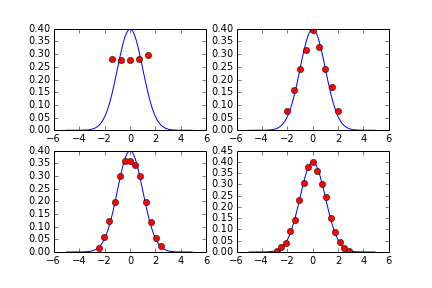
\includegraphics[width=120mm]{../programs/MC/central_limit_theorem/clt.png}
\caption{CLT for sampling with 1,2,3,4 states, respectively}
\end{figure}

\begin{figure}[ht!]
\centering
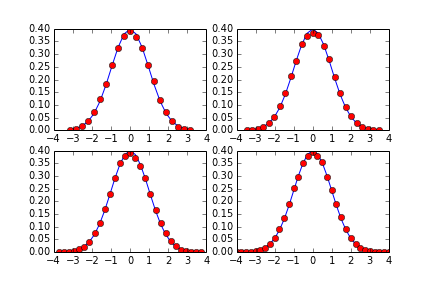
\includegraphics[width=120mm]{../programs/MC/central_limit_theorem/clt2.png}
\caption{CLT for sampling with 5,6,7,8 states, respectively}
\end{figure}

In the simulations of the Ising model we will be dealing with canonical distribution 
and we will be interested in the expectation values of various physical quantities. 
In the canonical distribution the system will have a probability distribution according 
to the Boltzmann weights. In the calculation, this probability distribution will be 
sampled and for each quantity we will apply CLT to estimate an error for its average 
value given by the standart deviation.

\chapter{The Monte Carlo Method (MC)}
\label{MC}

\section{Estimation of Expected Value} 

For a simulation of a system, the aim is to calculate expected value of a quantity. For instance, expected value of a quantity, Q, which follows Maxwell-Boltzmann distribution is 
$$
\langle Q \rangle = \frac{\sum\limits_{\mu} Q_\mu e^{-\beta E_\mu}}{\sum\limits_{\mu} e^{-\beta E_\mu}}
$$
where $\mu$ labels the state of the system and $\beta = \frac{1}{kT}$ and k is Boltzmann constant. 

By this method of calculating expected value of a quantity, all states of the system must be considered and this can be realized for systems with small number of states. However, when we consider larger systems, to calculate expected value of a quantity of system, a subset of these states must be used since all states cannot be considered. In this case, because of using a small portion of states, there will be an error in the calculated expected value. By Monte Carlo method, expected value of a large system can be calculated with low error. 

Monte Carlo method selects states of system, that is used to calculate expected value of a quantity, from a probabilty distribution, $P_\mu$ which we specify. With respect to Monte Carlo method, expected value of a quantity is

\begin{equation}
Q_M = \frac{\sum\limits_{i=1}^M {Q_\mu}_i {{P_\mu}_i}^{-1} e^{-\beta {E_\mu}_i}}{\sum\limits_{j=1}^M {{P_\mu}_j}^{-1} e^{-\beta{E_\mu}_j}}
\end{equation}

where states of system are $ \{ \mu_1, ..., \mu_M \} $ and $ Q_M $ is \textit{estimator of Q}. In the formulation, we see $ {{P_\mu}_i}^{-1} $ because we chose state  $ {Q_\mu}_i $ by a probability $ {P_\mu}_i $ from all of the states. 

Now, for an accurate estimation of expected value, $P_\mu$ must be defined. For instance, $P_\mu$ may be chosen as equal for all states. Then,

$$ Q_M = \frac{\sum\limits_{i=1}^M {Q_\mu}_i e^{-\beta {E_\mu}_i}}{\sum\limits_{j=1}^M e^{-\beta {E_\mu}_j}}$$


This is a poor choice for $P_\mu$. If probabilities of some states are greater than others, to get a good estimation of expected value, these states with high probabilities can	 be used. Therefore, equal $P_\mu$ for all states are not appropriate for this system, $P_\mu$ corresponding these states of high probabilities arranged to be high with respect to others. Hence, it is obvious that, if  $P_\mu$ is chosen in the form of Maxwell-Boltzmann distribution, then better approximation to expected value will occur.

When the number of states used to calculate expected value of a quantity by Monte Carlo method is increased, then estimator of Q converges to $\langle Q\rangle$. 

$$
\lim_{M \rightarrow \infty} Q_M = \langle Q \rangle
$$
\section{Sampling} 

To estimate expected value of a large system which has high number of states, Monte Carlo method should be used. For a system with states which has not equal probabilities, an appropriate $P_\mu$ must be defined, in order to approximate expected value of system. We have specified that if we choose $P_\mu$ in the form of Maxwell-Boltzmann distribution, then we get better approximation to expected value.

In this case, if we choose $P_\mu$ in the form,
\begin{equation}
P_\mu = Z^{-1} e^{-\beta E \mu} 
\end{equation}
then 
\begin{equation}
Q_M = \frac{1}{M} \sum\limits_{i=1}^M {Q_\mu}_i 
\end{equation}
 This sampling is called \textit{Importance Sampling}. Z is a normalization constant for probability $P_\mu$. In the following chapter, it is called \textit{Partition function}; since, if Z is known, then all macroscopic properties of a system can be calculated.

\section{Markov Process and Markov Chain} 

Now, the question is \textit{how} exactly we pick our states so that each one appears with its correct Maxwell-Boltzmann Probability. \cite[p. 34]{newman}. Hence, the problem is the generation of a random set of states according to a desired probability distribution which is Maxwell-Boltzmann distribution in statistical physics. 

\subsubsection{Markov Process}

Markov Process is a mechanism found by the Russian Mathematician Andrey Markov. In Markov Process, for a given state $\mu$, mechanism creates a new random state $\nu$. Probability to move state from $\mu$ to $\nu$ is \textit{Transition Probability}, $ P(\mu \rightarrow \nu) $.

Transition probabilities must satisfy two conditions:
Transition probabilities should be time independent and depend only on initial and final states, $\mu, \nu$, respectively. Also, it is obvious that,
\begin{equation}
\sum\limits_{\nu} P(\mu \rightarrow \nu) = 1 
\end{equation} 
which says that, sum of probabilities of transition from the state $\mu$ to other states $\nu$ and probability of staying in same state is equal to 1, as we expect.

\subsubsection{Markov Chain}

When simulating a system with Monte Carlo method, Markov Process is used repeatedly, as a chain, and a \textit{Markov Chain} is achieved. Simulation moves through the states, $\mu \rightarrow \nu \rightarrow \delta \rightarrow \lambda \rightarrow ...$. 

The Markov Process is chosen specially so that when it is run for long enough starting from any state, it will eventually produce a succession of states which appear with probabilities given by the Maxwell-Boltzmann distribution. 

First of all to get a stable distribution at the end of Markov chain, we should achieve equilibrium condition. Equilibrium condition states that, transitions into a state and out of that state must be equal. 

\newtheorem*{equil}{Equilibrium condition}
\begin{equil}
Thus, equilibrium condition can be written as following,
$$\sum\limits_{\nu} P_\mu P(\mu \rightarrow \nu) = \sum\limits_{\nu} P_\nu P(\nu \rightarrow \mu) $$
Therefore, 
$$P_\mu  = \sum\limits_{\nu} P_\nu P(\nu \rightarrow \mu)$$
\end{equil}

Hence, if above equation is satisfied at any step of Markov chain, then our probability distribution at the end of the Markov chain will be $P_\mu$. Now, we need a condition to achieve intended $P_\mu$ at equilibrium state. To achieve intended $P_\mu$, we should reach \textit{simple equilibrium}, by avoiding \textit{dynamic equilibrium}. 

%Hence, if above equation is satisfied with chosing transition probabilities sufficiently, equilibrium is achieved and $P_\mu$ will be the equilibrium probability value of the state $\mu$ at the end of the Markov chain. 
%Now, we need a condition to achieve equilibrium at the end of the Markov chain. To satisfy this equilibrium condition at the end, we should reach \textit{simple equilibrium}, by avoiding \textit{dynamic equilibrium}. 


\begin{enumerate}

\item Simple Equilibrium:

Let \textbf{P} is a matrix that consists of transition probabilities $P(\mu \rightarrow \nu)$, \textbf{P} is called \textit{Markov Matrix} or \textit{Stochastic Matrix} and let $\omega_\mu(t)$ is probability of system is in a state $\mu$ at time t. Then,
$$
 \omega_\nu(t+1) = \sum\limits_{\mu} P(\mu \rightarrow \nu) \omega_\mu(t) 
$$
With using matrix notation 
\begin{equation}
 \underline{\omega}(t+1) = \textbf{P} \underline{\omega}(t)
\end{equation}
$\underline{\omega}(t) $ is an array consists of $\omega_\mu(t)$. 

If simulation reaches simple equilibrium, then 
\begin{equation}
\underline{\omega}(\infty) = \textbf{P} \underline{\omega}(\infty) 
\end{equation}

In this case, $\underline{\omega}(\infty)$ equals Maxwell-Boltzmann distribution, by choosing appropriate probabilities.

\item Dynamic Equilibrium:

If we reach dynamic equilibrium, probability distribution $\omega$ rotates around different values. This rotation is called \textit{limit cycle}. If we are in a limit cycle 
\begin{equation}
\underline{\omega}(\infty) = \textbf{P}^n \underline{\omega}(\infty) 
\end{equation}
where n is the length of limit cycle. To get rid of dynamic equilibrium, we should satisfy \textit{Detailed balance} condition.

\end{enumerate}

\begin{enumerate}

\item Detailed Balance:

Using detailed balance, we obtain Maxwell-Boltzmann distribution rather than any distribution, after achieving the equilibrium condition, .

\newtheorem*{balance}{Detailed Balance}
\begin{balance}
$$ P_\mu P(\mu \rightarrow \nu) = P_\nu P(\nu \rightarrow \mu)$$
\end{balance}

Detailed balance condition forbids dynamic equilibrium, clearly. For instance, we have a probability for a state and this probability will increase at a step of limit cycle, to increase this probability, we must have more transitions to this state than out of it, on average; however, detailed balance blocks it. Hence, with using detailed balance, we can get rid of dynamic equilibrium.

If we look at detailed balance condition, it also includes equilibrium condition which is described above. Hence, if detailed balance is satisfied, then equilibrium condition will be satisfied and we will avoid to get dynamic equilibrium and limit cycles. 

Once we remove limit cycles in this way (by using detailed balance), it is straightforward to show that the system will always tend to the probability distribution $P_\mu$ as $t \rightarrow \infty $. \cite[p. 38]{newman}. It means that $\omega_\mu(\infty) = P_\mu$.

Let's show that the system tend to $P_\mu$ as $t \rightarrow \infty $;

It is known that, $  \underline{\omega}(t+1) = \textbf{P} \underline{\omega}(t)$. If t is chosen to be equal to zero, we will get  $  \underline{\omega}(1) = \textbf{P} \underline{\omega}(0)$ and by making some iterations, then
\begin{equation}
\underline{\omega}(t) = \textbf{P}^t \underline{\omega}(0)
\end{equation}

Also, $  \underline{\omega}(0) $ can be expressed as a linear combination of eigenvectors $\underline{v_i}$ of \textbf{P}, \cite[p. 66]{newman}
\begin{equation}
\underline{\omega}(0) = \sum\limits_{i} a_i\underline{v_i} 
\end{equation}


Then $$  \underline{\omega}(t) = \textbf{P}^t \sum\limits_{i} a_i\underline{v_i} $$ Also, we know that $ \textbf{P} \underline{v_i} = \lambda_i \underline{v_i} $ where $ \lambda_i $ is eigenvalue corresponding eigenvector $ \underline{v_i} $. Then, 
\begin{equation}
\underline{\omega}(t) = \sum\limits_{i} a_i {\lambda_i}^t \underline{v_i} 
\end{equation}


%As t goes to $\infty$, ${\lambda_i}^t$ grows with t and equation will be dominated by largest eigenvalue $\lambda_0$ of \textbf{P}. Hence, as t goes to $\infty$, $\omega(t)$ becomes proportional to $\underline{v_0}$ which is eigenvector corresponding to $\lambda_0$.

%Therefore, $\omega(t)$ approximates exponentially to eigenvector corresponding largest eigenvalue of \textbf{P}.

Besides, we know that $\sum\limits_{\nu} P(\mu \rightarrow \nu) = 1 $. Thus, sum of all elements in each column of Markov matrix equals to 1. On the other hand, since elements of Markov matrix describes probabilities, they are in the range [0,1]. 

%Also, $\omega(t)$ is a probabilty vector, that contains probabilities of each state at time t. Hence, sum of each elements of %$\omega(t)$ equals to 1.  

Let's assume a 2x2 Markov Matrix \textbf{P}; 
\[\begin{bmatrix}
a&b\\
1-a&1-b\\  
\end{bmatrix}\]

and transpose of \textbf{P} is $\textbf{P}^T$
\[\begin{bmatrix}
a&1-a\\
b&1-b\\  
\end{bmatrix}\]

To find its eigenvectors and eigenvalues  $\textbf{P}^T v_i = \lambda_i \underline{v_i} $ then, ($\textbf{P}^T - \lambda_i I) \underline{v_i}  =0  = \textbf{K} \underline{v_i} $ then \textbf{K} is
\[\begin{bmatrix}
a-\lambda&1-a\\                   
b&1-b-\lambda\\  
\end{bmatrix}\]

Hence, generally for the transpose of a n by n Markov Matrix $\textbf{P}$, eigenvector $\underline{v_i} $ is
\[\begin{bmatrix}
1\\ 
1\\ 
\vdots\\ 
1 
\end{bmatrix}\]

and for this eigenvector which has elements of 1, there is an eigenvalue of 1. To see this, using same 2x2 Markov Matrix, and $\textbf{P}^T \underline{v_i} = \lambda_i \underline{v_i} $;
$ a - \lambda + 1 - a = 0 \qquad b + 1 - b - \lambda = 0 $ then $\lambda =1 $.

Markov Matrix , \textbf{P}, and its transpose have same determinant, then  $\textbf{P} - \lambda I $ and $ \textbf{P}^T - \lambda I $ have same determinant. Hence, eigenvalues of \textbf{P} and $\textbf{P}^T $ are same (because determinants are equal). Therefore, Markov Matrix \textbf{P} has an eigenvalue of 1.

Now, let's assume $v_i$ is an eigenvector corresponding to eigenvalue $| \lambda| > 1$ and $\textbf{P}^n \underline{v_i} =  | \lambda |^n \underline{v_i} $, so its lenght grows exponentially for n goes to $\infty$. Hence, for a large n, an element of $\textbf{P}^n$ must be larger than one (to satisfy equality), which is impossible. So, all eigenvalues of \textbf{P} is small or equal to 1.

Also, we have found $$ \underline{\omega}(t) = \sum\limits_{i} a_i {\lambda_i}^t \underline{v_i} $$ as t goes to $\infty$ eigenvalues which has an absolute value is smaller than 1 vanishes and right hand side of equation dominated by eigenvalue $\lambda_0 = 1 $. Hence, for a long time $\underline{\omega}(t)$ is proportional to $\underline{v_0}$ which is eigenvector corresponding $\lambda_0$ that has elements of 1. Hence,
\begin{equation}
 \underline{\omega}(\infty) = a_0 \underline{v_0}
\end{equation}

Besides, in equilibrium, we have that $P_\mu = \sum\limits_{\nu} P_\nu P(\nu \rightarrow \mu)$ with vector notation, it is equal to $\underline{p} = \textbf{P} \underline{p}$. \underline{p} is a vector whose elements are $P_\mu$. For an eigenvalue and a corresponding eigenvector of matrix \textbf{A}, $\textbf{A} \underline{v} = \lambda \underline{v}$ Hence, if we write $$\textbf{P} \underline{p} = \lambda \underline{p} $$, then \underline{p} is a normalized eigenvector of \textbf{P} which has eigenvalue 1. It means that $\underline{v_0} = \underline{p}$


Therefore, $\underline{\omega}(\infty) $ is $\underline{p}$, because of that, when t goes to infinity, $\underline{\omega}(t)$ goes to $\underline{p}$.
\begin{equation}
\lim_{t \rightarrow \infty} \underline{\omega}(t) = \underline{p}
\end{equation}



By carefully choosing transition probabilities which satisfy detailed balance condition, we can reach any probability distribution $\underline{p}$ in equilibrium.


Now, we want to satisfy Maxwell-Boltzmann distribution in equilibrium condition, therefore we choose $p_\mu$ as the Maxwell-Boltzmann probabilities. By using detailed balance condition;
\begin{equation}
\frac{P(\mu \rightarrow \nu)}{P(\nu \rightarrow \mu)} = \frac{P_\nu }{P_\mu } = e^ {-\beta (E_\nu - E_\mu)}
\end{equation}


Also, to show all states must be a part of the system, we should satisfy \textit{Ergodicity} condition.

\item Ergodicity:

With respect to condition of ergodicity, some of transition probabilities may be zero, however through any two states, which has transition probabilty equals to zero, there must be at least one path of non-zero probability. Thus, all states in the system must be reachable by at least one path, it means that all states must be a part of the system.

Therefore, we have to satisfy three conditions:
\begin{enumerate}
\item $\frac{P(\mu \rightarrow \nu)}{P(\nu \rightarrow \mu)} = \frac{P_\nu }{P_\mu } = e^ {-\beta (E_\nu - E_\mu)}$
\item $\sum\limits_{\nu} P(\mu \rightarrow \nu )  =1 $
\item Ergodicity

\end{enumerate}


If these three conditions are satisfied, then we get Maxwell-Boltzmann distribution as an equilibrium distribution.

There are a lot of transition probabilities to satisfy these conditions. There is a lot of algorithms to realize it such as \textit{Metropolis algorithm}. However, a purpose-built algorithm can often give a much faster simulation than an equivalent standard algorithm, and the improvement in efficiency can easily make the difference between finding an answer to a problem and not finding one. \cite[p. 40]{newman}

\end{enumerate}


\section{Acceptance Ratio and Selection Probabilities} 

We have two equations to satisfy, one is the ratio of transition probabilities and the other is the sum of transition probabilities to move a state to other states. 

Let's consider "stay-at-home" condition $\nu = \mu$, then ratio of transition probabilities equals 1, so first condition (detailed balance) is satisfied, independent of $P(\mu \rightarrow \mu)$. So, we can choose other transition probabilities more easily. This flexibilty comes from the $\sum\limits_{\nu} P(\mu \rightarrow \nu )  =1 $, we can adjust any $P(\mu \rightarrow \nu)$. For an adjustment in  $P(\mu \rightarrow \nu)$, we can adjust $P(\nu \rightarrow \mu)$ to keep the ratio constant. So, by changing  $P(\mu \rightarrow \mu)$, we can use any value of $P(\mu \rightarrow \nu)$. 

Let's assume $$P(\mu \rightarrow \nu) = g(\mu \rightarrow \nu) A(\mu \rightarrow \nu) $$ where, $g(\mu \rightarrow \nu)$ is the \textit{Selection probability}, which is the probabilty of generating new state and $A(\mu \rightarrow \nu)$ is the \textit{Acceptance Ratio}. It represents that if our algortihm creates a new state $\nu$, then with a fraction of time $A(\mu \rightarrow \nu)$ we will accept that new state $\nu$ and we will stay in first state at the rest of time. Acceptance ratios are about the "stay-at-home" conditions, for example if we choose $A(\mu \rightarrow \nu) = 0$ for all $\nu$ then $P(\mu \rightarrow \mu) = 1$, because if we don't accept any move to another state, then our "stay-at-home" probability is 1. So we are free to choose any value of $A(\mu \rightarrow \nu) $ in between 0 and 1.

If we look at the equation $\frac{P(\mu \rightarrow \nu)}{P(\nu \rightarrow \mu)} = \frac{P_\nu }{P_\mu } = e^ {-\beta (E_\nu - E_\mu)}$, then we have a constraint in $$\frac{P(\mu \rightarrow \nu)}{P(\nu \rightarrow \mu)} = \frac{g(\mu \rightarrow \nu)A(\mu \rightarrow \nu)}{g(\nu \rightarrow \mu)A(\nu \rightarrow \mu)} $$

We can choose any value of $\frac{A(\mu \rightarrow \nu)}{A(\nu \rightarrow \mu)}$ and this gives us a freedom in the value of $g(\mu \rightarrow \nu) $ and $g(\nu \rightarrow \mu) $. Hence, we will create a MC algorithm that creates new states with probabilities $g(\mu \rightarrow \nu) $ and then we will accepts it with probabilities $A(\mu \rightarrow \nu) $.

However, there is also a requirement in the values of $A(\mu \rightarrow \nu) $. If we choose acceptance ratios to be low, then we cannot generate enough states. Thus, we want to choose $A(\mu \rightarrow \nu) $ as close as to unity. For chosen selection probabilities, we only have a constraint on the ratio $\frac{A(\mu \rightarrow \nu)}{A(\nu \rightarrow \mu)}  $. Hence, we choose largest acceptance ratios as 1, that implies, for example,  $A(\mu \rightarrow \nu) = 1 $, and the other is fixed by the ratio of acceptance probabilities.



\chapter{The Ising Model and two of its MC Algorithms}

\section{The Ising Model}

The Ising model is a model of magnetization of a material. The magnetization of a material is formed by magnetic dipole moments of spins. Ising models material as a lattice which includes spins. Spin can be +1 or -1 and it is represented by $s_i$. +1 or -1 spins stand for up-pointing or down-pointing dipoles. For a system which has N spins, there are $2^N$ total states. These spins interact with each other. We consider the simplest case, all interactions has the same strength, which is represented by J (interaction energy), and the interactions occurs only between the neighbouring spins. Also, we can deal with an external magnetic field acting on spins in this simplest case.
In this case Hamiltonian \texttt{H} is; 
\begin{equation}
\texttt{H} = - J \sum\limits_{<i,j>} s_i s_j - H\sum\limits_{i} s_i
\end{equation}
We know that, Hamiltonian of Ising model represents Energy of system.
Partition function of the Ising model is 
\begin{equation}
Z = \sum\limits_{\{s_i\}} e^{-\beta \texttt{H}}
\end{equation}
$\{s_i\}$ means that we actualize the sum for all spins and for all values of spins, which are $+1$ and $-1$. Hence, $\{s_i\}$ represents all possible microstates of the Ising model.

If a large system, which has a fixed volume and fixed number of particles, is in interaction with environment, then we call this system \textit{cannonical ensemble}. Canonical partition function for an cannonical ensemble is $ Z = \sum\limits_{\{i\}} e^{-\beta E_i} $ where $i$ is the microstate of the system and $E_i$ is the energy at that state. Also, $    \beta = \frac{1}{kT}$. 

As previously defined, Z is a normalization constant for $P_\mu$ and macroscopic properties of system can be calculated by using Z.

We know that expectation of a quantity is $ \langle Q \rangle = \frac{\sum\limits_{\mu} Q_\mu e^{-\beta E_\mu}}{\sum\limits_{\mu} e^{-\beta E_\mu}}$ which follows Maxwell-Boltzmann distribution. We can write it in terms of Z
\begin{equation}
\langle Q\rangle = \frac{1}{Z}\sum\limits_{\mu} Q_\mu e^{-\beta E_\mu}
\end{equation}
Expectation value of energy is internal energy U. 
\begin{equation}
\langle E\rangle = U = \frac{1}{Z} \sum\limits_{\mu} E_\mu e^{-\beta E_\mu} = -\frac{1}{Z} \frac{\partial Z}{\partial \beta} = -\frac{\partial logZ}{\partial \beta}
\end{equation}
Specific heat, C, is the required heat to increase the temp one degree. Thus,
\begin{equation}
C = \frac{\partial U}{\partial T} = \frac{\partial U}{\partial \beta} \frac{\partial \beta}{\partial T} = \left[ - \frac{\partial^2 logZ}{\partial \beta^2}    \right] \left[ -k \beta^2       \right] = k \beta^2 \frac{\partial^2 logZ}{\partial \beta^2}
\end{equation}
Entropy, S, is defined as 
\begin{equation}
C = T \frac{\partial S}{\partial T} = -\beta \frac{\partial S}{\partial \beta}
\end{equation}
\begin{equation}
S = - k \beta \frac{\partial logZ}{\partial \beta}  + k log Z
\end{equation}

(There is also a constant in S but according to the 3rd law of Thermodynamics it is 0.)
Helmholtz free energy, F, is defined as,
\begin{equation}
F = U - TS = -kTlogZ
\end{equation}
Pressure, p, is conjugate variable of volume V. Hence,
\begin{equation}
p = - \frac{\partial F}{\partial V}
\end{equation}
Also, magnetization, M, is conjugate variable of magnetic field. Thus,
\begin{equation}
M = \frac{\partial F}{\partial H}
\end{equation}
Then, we can calculate magnetic susceptibility, $\chi$ by
\begin{equation}
\chi =\frac{\partial \langle M \rangle}{\partial H}
\end{equation}

We will simulate the Ising model with Monte Carlo Method with using two different algorithms.

\section{Macroscopic Properties of Ising Model}

In this section, we will look at the properties of Ising model that will be studied in Monte Carlo simulations. In the Monte Carlo simulations, we will calculate:
\begin{enumerate}[start=1]

\item Magnetization per site

Instead of calculating magnetization with using free energy, we will calculate it more easily. 

Mean magnetization per site can be calculated using, 
\begin{equation}
\langle m \rangle = \frac{1}{N} \left\langle \sum\limits_{i} s_i \right\rangle
\end{equation}

\item Internal Energy per site

Instead of calculating internal energy with using partition function, we will calculate it with using definition of energy.

Internal energy per site can be calculated using, 
\begin{equation}
u = \frac{1}{N} \langle H_E \rangle = \frac{1}{N} \langle - J \sum\limits_{<i,j>} s_i s_j - H \sum\limits_{i} s_i \rangle
\end{equation}

\item Specific Heat per site 

Specific heat per site is defined as $c = \frac{1}{N} \frac{\partial U}{\partial T} =\frac{k \beta^2}{N} \frac{\partial^2 logZ}{\partial \beta^2}$
\begin{equation}
c = \frac{k \beta^2}{N} \frac{\partial}{\partial \beta} \left(  \frac{1}{Z} \frac{\partial Z}{\partial \beta}     \right) = \frac{k \beta^2}{N} \left[ \frac{1}{Z} \frac{\partial^2 Z}{\partial \beta^2} - \frac{1}{Z^2} \left( \frac{\partial Z}{\partial \beta}\right)^2 \right] = \frac{k \beta^2}{N} [ \langle E^2 \rangle - \langle E \rangle^2 ]
\end{equation}
where
\begin{equation}
\langle E^2 \rangle = \frac{1}{Z}\sum\limits_{\mu} {E_\mu}^2 e^{-\beta  E_\mu} = \frac{1}{Z} \frac{\partial^2 Z}{\partial \beta^2}   
\end{equation}
Also,
\begin{equation}
c = k \beta^2 N [ \langle E_{ps}^2 \rangle - \langle E_{ps} \rangle^2 ]
\end{equation}

where $E_{ps}$ is energy per site.

\item Magnetic Susceptibility per site

Magnetic susceptibility per site is defined as $ \chi = \frac{1}{N} \frac{\partial \langle M \rangle}{\partial H} $ 

If we use Fluctuation Dissipation Theorem for Magnetic susceptibility we get 
\begin{gather}
\chi = \frac{\beta}{N} [ \langle M^2 \rangle - \langle M \rangle^2    ] \\
\chi = \beta N [ \langle m^2 \rangle - \langle m \rangle^2    ]
\end{gather}

\end{enumerate}

\section{How to Analyze Properties with Monte Carlo Method }

Now, we know how to calculate magnetization per site and energy per site for Ising model in a Monte Carlo simulation for any state of system with considering only spins in that state. After calculation magnetization per site and energy per site, we can calculate the mean of them. Also, other two properties of the system, specific heat and magnetic susceptibility, are depend on the fluctations on the magnetization and energy. Hence, to calculate them, we have to analyze magnetization and energy, previously. 

\subsection{Equilibration Time}

To ensure that our states follow Maxwell-Boltzmann distribution, we have to make sure that we are in equilibrium. Hence, after the simulation started, to make observations of system properties, we should wait a period of time for the system to reach equilibrium. This time period is called equilibration time $\tau_{eq}$. When equilibrium is achieved, the  probability of the system being in a state is proportional to Maxwell-Boltzmann distribution. 

As previously defined, when equilibrium is reached, the system spends most of the time in states which have small range of energies. Hence, to see the system to get equilibrium, we can observe energy or magnetization.


\subsection{Autocorrelation Function and Correlation Times}

If we want to analyze system more efficiently, we should use independent data in our simulation. Hence, to get independent data from the simulation, we should use states which are independent from each other. To get independent states, we have to wait a period of time between two independent state, this period of time is called  \textit{Correlation time} $\tau$ of simulation after system has achieved the equilibrium. Correlation time is a measure of how long it takes the system to get from one state to another one which is significantly different from the first. \cite[p. 59] {newman}. To calculate correlation time, time displaced autocorrelation function should be considered.

\subsubsection{Time Displaced Autocorrelation Function}

For example, let's consider the quantity magnetization. Time-Displaced Autocorrelation $\chi (t)$ of magnetization is;

\begin{equation}
\chi (t) = \int dt' [m(t') - \langle m\rangle][m(t' + t) - \langle m\rangle] = \int dt'[m(t')m(t' + t) - {\langle m\rangle}^2]
\end{equation}

where, m(t) is magnetization at time t.  $\chi (t) $ gives correlation of two different values of magnetization with t time difference. If $\chi (t) \neq 0$, then on average, the fluctations are correlated, otherwise, uncorrelated. 

Autocorrelation is expected to fall off exponential; hence,
\begin{equation}
\chi (t) \sim e^{-t/ \tau}
\end{equation}
where $\tau$ is the correlation time.

When t = $\tau$ , $\chi (\tau) = 1/e = 0.367879 $, this is still an high value.  Hence, the time needed for independent samples is greater then correlation time. For some considerations, this time is chosen as $2\tau$. This is came from some analysis in error calculation.

There are three basic ways to determine correlation time;

Autocorrelation function is an exponential decaying function, Hence it has its maximum value when t=0. If the autocorrelation function is normalized with its value at t=0, then the max value of this function is 1, at t=0. Then, if $\frac{\chi (t)}{\chi (0)}$ is plotted with respect to t; then, correlation time can be found by searching the value  $\frac{\chi (t)}{\chi (0)} = \frac{1}{e}$. 

Also, correlation time may be calculated with using \textit{Integrated Correlation time}
\begin{equation}
\int\limits_{0}^{\infty} \frac{\chi (t)}{\chi (0)} dt =\int\limits_{0}^{\infty} e^{-t/ \tau} dt = \tau
\end{equation}

Another way to find correlation time is to plot logarithm of normalized autocorrelation function with respect to t, logarithm of normalized autocorrelation function is $log(\frac{\chi (\tau)}{\chi (0)}) = \frac{-t}{\tau}$. Then, by finding the slope of the plot, we can measure correlation time. The slope is equal to $\frac{-1}{\tau}$. 

To practise autocorrelation function in the simulation, autocorrelation function should be calculated in discrete time domain. 
\begin{equation}
\chi (t) = \frac{1}{t_{max} - t} \sum\limits_{\nu = 0 }^{t_{max} - t} m(t')m(t' + t ) - \frac{1}{t_{max} - t} \sum\limits_{\nu = 0 }^{t_{max} - t} m(t') * \frac{1}{t_{max} - t } \sum\limits_{\nu = 0 }^{t_{max} - t} m(t' + t)
\end{equation}
Then $\chi (t) / \chi (0)$ should be plotted. Then, with above analysis, we can determine correlation time. However, this formula to calculate autocorrelation function takes time proportional to $n^2$ where n equals to number of samples. 

To decrease this time, Fourier Transform of the autocorrelation function should be calculated. Then, by taking inverse Fourier Transform, autocorrelation function can be calculated.

Fourier Transform of autocorrelation function;
\begin{equation}
\chi_{FT}(\omega) = \int dte^{i\omega t} \int dt'[m(t') -\langle m\rangle][m(t' + t) - \langle m\rangle] 
\end{equation}
With using \textit{Cross-Correlation Theorem} of Fourier Transform 
\begin{equation}
\chi_{FT} (\omega) = \mid m'_{FT} (\omega) \mid ^2
\end{equation}
where $m'_{FT} (\omega)$ is Fourier Transform of $m'(t) = m(t) - \langle m\rangle$ 

Fourier Transform of $m'(t)$ can be calculated using \textit{Fast Fourier Transform (FFT)}.  Hence, firstly FFT of $m'(t)$ should be taken and $\chi_{FT}(\omega)$ should be calculated with given function. Then taking Inverse FFT of $\chi_{FT}(\omega)$, $\chi (t)$ can be found.  After that, correlation time can be calculated with normalizing  $\chi (t) $ and using above one of the methods to find correlation time. 

Also, if $\langle m\rangle$ is calculated over a much longer run than $\chi_{FT} (\omega)$, then correlation time can be found without taking inverse FFT.\cite[p. 65]{newman}. From the definiton of the Fourier Transform;
\begin{equation}
\chi_{FT} (0) = \int \limits_{0}^\infty \chi (t)dt = \tau \chi (0)
\end{equation}
then,
\begin{equation}
\tau = \frac{\chi_{FT} (0)}{\chi (0)}
\end{equation}
where, $\chi (0) = \langle m^2\rangle  - \langle m\rangle^2$, which is variance in magnetization.

\subsubsection{Correlation Times and Markov Matrices}

There are a lot of correlation times which correspond to every state of the system. As previously mentioned,  $ \underline{\omega}(t+1) = \textbf{P} \underline{\omega}(t) $ where , $ \underline{\omega}(t)$ is a vector of probabilities of finding the states. By iteration $  \underline{\omega}(t) = \textbf{P}^t \underline{\omega}(0)$. 
Also, $\underline{\omega}(0)$ can be expressed as a linear combination of eigenvectors of $\textbf{P}$, $\underline{\omega }(0) = \sum\limits_{i} a_i \underline{v_i} $. Then $  \underline{\omega}(t) = \textbf{P}^t \sum\limits_{i} a_i\underline{v_i} $. Also, we know that $ \textbf{P} \underline{v_i} = \lambda_i \underline{v_i} $ where $ \lambda_i $ is eigenvalue corresponding eigenvector $ \underline{v_i} $. Then, $ \underline{\omega}(t) = \sum\limits_{i} a_i {\lambda_i}^t \underline{v_i} $.

As t goes to $\infty$, largest eigenvalue, $\lambda_0$ of $\textbf{P}$ dominates. Then, $\underline{\omega}(t) $ is proportional to $v_0$ which is eigenvector corresponding the largest eigenvalue. Also, $\underline{\omega}(t)$ tends to Maxwell-Boltzmann distribution. 
\begin{equation}
\underline{\omega}(\infty) = a_o \underline{v_0}
\end{equation}

Expectation value of a quantity Q at time t is 
\begin{equation}
Q(t) = \sum\limits_{\mu} \omega_\mu (t) Q_\mu = \underline{q} \underline{\omega}(t)
\end{equation}
Then,
\begin{equation}
Q(t) = \sum\limits_{i} a_i {\lambda_i}^t \underline{q} \underline{v_i} = \sum\limits_{i} a_i {\lambda_i}^t q_i
\end{equation}
where, $q_i = \underline{q} \underline{v_i}$ , $q_i$ is the expectation value of Q in the $i^{th}$ eigenstate.

As t goes to $\infty$, $ Q(\infty)  = a_0 q_0$, $Q(\infty)  $ is proportional to $q_0$ denoted by $\lambda_0$. By defining,
\begin{equation}
\tau_i = \frac{-1}{log \lambda_i} ,  i \neq 0
\end{equation}
then,
\begin{equation}
Q(t) = a_0 q_0 + \sum\limits_{i \neq 0 } a_i q_i e^{\frac{-t}{\tau_i}} = Q(\infty) +\sum\limits_{i \neq 0 } a_i q_i e^{\frac{-t}{\tau_i}}
\end{equation}
where, $\tau_i$'s are the correlation times for system. Also, $Q(\infty)$ is the equilibrium expectation $\langle Q\rangle$.

Autocorrelation function of Q can be written as,
\begin{equation}
\chi (t) = [Q(0) - Q(\infty)][Q(t) - Q(\infty)] = \sum\limits_{i \neq 0} a_i q_i \sum\limits_{i \neq 0} a_i q_i e^{\frac{-t}{\tau_i}}
\end{equation}
Then,
\begin{equation}
\chi (t) = \sum\limits_{i \neq 0} b_i e^{\frac{-t}{\tau_i}}
\end{equation}
where, $b_i = \sum\limits_{j \neq 0 } a_i a_j q_i q_j$

This is the generalization of $\chi (t) \sim e^{\frac{-t}{\tau}}$ for all times, not only for long times. Hence, there are as many correlation times as the eigenvalues, or eigenstates.  Since, rank of matrix \textbf{P} is equal to states of system, there are as many correlation times as the states of the system. Actually, this is 1 less from the states of system, because if we look at the definition of $\tau_i$ there is no $\tau_0$. For example, for Ising model there are $2^N$ states, hence, there are $2^N - 1 $ correlation times. The longest correlation time is $\tau_1$ which corresponds to $\lambda_1$ which is the second largest eigenvalue. In previous subsection, this is labelled as $\tau$. For long simulation times, we only pay attention to this $\tau_1$ because, if we look at $ \chi (t) = \sum\limits_{i \neq 0} b_i \lambda_i^t$, all $\lambda^t$'s will die away and largest $\lambda$ will be predominate. (We knew that all $\lambda$'s are smaller than 1 except for $\lambda_0$.)

In general the most accurate results are obtained by fitting our autocorrelation function to sum of a small number of decaying exponentials, choosing values for the quantities $b_i$ by a least-squares or similar method.\cite[p. 67]{newman}

Hence, to find correlation time $\tau$ for any temperature, autocorrelation function of a quantity may be examined after the equilibrium is achieved. Hence, calculating autocorrelation function for all quantities that we are interested and using maximum of the correlation times is a good choice for us. 

Now, we have independent data for quantities after reaching the equilibrium. Hence, with using these, we can examine fluctations in these quantities to analyze other macroscopic properties of the system. However, previously, we should determine our error ranges in these quantities.

\subsection{Errors in Calculation}

To make a complete analysis, we have to determine tolerances in our datas. Errors on Monte Carlo results can be divided into 2 classes: Statistical errors and Systematic errors. Statistical errors are result of randomness in Monte Carlo simulations and these errors can be decreased by taking a lot of samples. Systematic errors are caused by the alghorithm that is used to make measurements.

\subsubsection{Statistical Errors}

In a Monte Carlo calculation, value of a quantity changes from step to step, 
as a result of randomness. It is often straightforward to estimate the 
statistical error in a measured quantity, since the assumption that the error 
is statistical implies that we can estimate the true value by taking the mean 
of several different measurements, and that the error on that estimate is 
simply the error on the mean. \cite[p. 68]{newman}

The basic error analysis of a statistical measurement is direct calculation of 
standard deviation of measurement: 

For example, take n measurements of a quantity $q_i$. Mean of that 
quantity is $\langle q \rangle$ . Then, error is 
\begin{equation}
\sigma = \sqrt{\frac{\frac{1}{n} \sum\limits_{i=0}^n (q_i - \langle q 
\rangle )^2}{n-1}} = \sqrt{\frac{1}{n-1} ( \langle q^2 \rangle - \langle 
q\rangle^2)}
\end{equation}
It is known that $n = \frac{t_{max}}{2\tau} >> 1$ then,

\begin{equation}
\sigma = \sqrt{\frac{2\tau}{t_{max}} (\langle q^2\rangle - \langle 
q\rangle^2)}
\end{equation}

Besides, there are four error analysis methods for an statistical 
measurement: 

\begin{enumerate}

\item The Blocking Method

In the Blocking Method, data is  divided in to several blocks with several 
samples and for each block, mean of that quantity is calculated. Then, 
putting them into the 

\begin{equation}
\sigma = \sqrt{\frac{\frac{1}{n} \sum\limits_{i=0}^n (q_i - \langle q 
\rangle )^2}{n-1}} = \sqrt{\frac{1}{n-1} (\langle q^2 \rangle - \langle 
q\rangle^2)}
\end{equation}

where, this time n is block number and q is the mean of the quantity.  

\item The Bootstrap Method

When calculating a quantity of the system, independent samples are chosen 
in data of that quantity. In the Bootstrap method, we resample these 
quantity, again we choose n samples from that data values but this time, 
these n samples are chosen randomly; also, these samples can be same, 
and using these n samples we calculate that quantity. In this case, n can be 
any value, for example, number of independent samples of that quantity. 
This procedure is repeated for i times and for each time we calculate the 
quantity $q_i$. Then, error in that quantity is the standart deviation in the 
values $q_i$, which is 
\begin{equation}
\sigma= \sqrt{\langle q^2 \rangle - \langle q \rangle^2}
\end{equation}

\item The Jackknife Method

When calculating a quantity, n independent samples are used. In the 
Jackknife method, that quantity is calculated again with using n-1 samples 
by removing first, second, ... ith independent sample, respectively, if 
quantities are labeled as $q_i$ with ith sample removed, then 
\begin{equation}
\sigma = \sqrt{\sum\limits_{i=1}^n (q_i - q )^2}
\end{equation}

where, q is the quantity calculated with n samples. 




( YENI)



\item The Bunching Method

To calculate error in a quantity, we can calculate standard deviation in data 
after bunching data into;:
$$(q_0 + q_1)/2,(q_2 + q_3)/2, ... , (q_{n-2} + q_{n-1})/2 $$
Then, again we can calculate standard deviation after bunching this data 
$$[(q_0 + q_1)/2 + (q_2 + q_3)/2]/2, ...
, [(q_{n-4} + q_{n-3})/2 + (q_{n-2} + q_{n-1})/2]/2$$
By iterating this process, we can calculate standard deviation for each 
iteration.  Actually, this is a very similar method to blocking method, the 
only difference is that we are blocking data several times.





Hesap yapılırken kok n-1 yerine kok n kullanıldı. Fark ne? onceden niye kok 
n-1 di. clt ye gore kok n olmasını bekliyoruz.

(SON)




\end{enumerate}

\subsubsection{Systematic Errors}

For systematic errors, there is no general method of estimate. There are 2 obvious systematic errors in Metropolis simulation of the Ising Model. Firstly, to reach the equilibrium state, we wait a finite amount of time. Actually, we get Maxwell-Boltzmann distribution when t goes to infinity. The other error is that not running the simulation long enough after equilibrium to take independent samples.

\section{Metropolis Algorithm}

To derive Metropolis algorithm, firstly, we choose $g(\mu \rightarrow \nu)$ and in oder to satisfy detailed balance condition we choose appropriate $A(\mu \rightarrow \nu)$ and the algorithm chooses a new state $\nu$ and then accepts or rejects it with respect to the acceptance ratio, and if it accepts, we move to the new state, else we stay at the current state and the algorithm repeats itself. $g(\mu \rightarrow \nu)$ should be arranged to satisfy Ergodicity condition. 

Mean of energy is U. $E[E] = \mu_E = \langle E \rangle = U$ Then, variance in energy is $\sigma^2 = E[(E-\mu_E)^2] = E[E^2] - {\mu_E}^2$. We have shown that $$ 
U = E[E] = - \frac{\partial \log Z}{\partial \beta}
$$
and 
$$
E[E^2] = \frac{1}{Z} \frac{\partial^2 Z}{\partial \beta^2}
$$
Hence, 
\begin{equation}
Var[E] = E[E^2] - (E[E])^2 = \frac{\partial^2 \log Z}{\partial \beta^2}
\end{equation}
Then, standart deviation $\sigma_\epsilon$ is
\begin{equation}
\sigma_\epsilon = \sqrt{\frac{\partial^2 \log Z}{\partial \beta^2}}
\end{equation}

The variation of the actual value of U around the expectation value $\mu_E$ is tiny by comparison with the kind of energies we are considering for the whole system, and probably not within the resolution of our measuring equipment.\cite[p. 11]{newman}

So, energy fluctations are the very small portion of the total energy. This means that, system mostly in states with a narrow range of energy.Thus, in the simulation, we want to be in that states, mostly. An algorithm which has \textit{Single-spin-flip dynamics} is an algorithm for this case. 


Single-spin-flip dynamics state that, maximum energy difference between new state $\nu$ and current state $\mu$ is 2J for each bond between spin we flip and its neighbours.  For example, in 2D lattice a site has 4 neighbours then maximum difference between energies of 2 states is 8J.  Therefore, in general, maximum energy difference between states is $2zJ$ where z is the lattice coordination number, which means that number of neighbours of a site. Also, single-spin-flip dynamics guarantees the ergodicity condition. For any state, there is always a chance to go to that state from current state.

Let's look at the Metropolis Algortihm. According to the Metropolis Algorithm, $g(\mu \rightarrow \nu)$ is same for all possible states $\nu$. For instance, for a system with N states, that we can access from current state $\mu$, $g(\mu \rightarrow \nu) = \frac{1}{N}$
In this case, to satisfy detailed balance condition: 
\begin{equation}
\frac{A(\mu \rightarrow \nu)}{A(\nu \rightarrow \mu)} = e^{-\beta (E_\nu - E_\mu) }
\end{equation}

There is no condition for the individual acceptance ratios. Therefore, for example, we can choose $A(\mu \rightarrow \nu) = A_0 e^{ - \frac{1}{2} \beta (E_\nu - E_\mu)}$ and we can set $A_0$ to be any value with considering acceptance ratio is a probabilty value. However, this choice of acceptance ratio is inefficient. Because, we have low probabilities to accept a move and in this case we generally do not move to another site. 

To maximize acceptance ratio, as earlier mentioned, we set larger of two acceptance ratios to 1, by changing $A_0$ and adjust the other to satisfy detailed balance condition. 

For insance, let $E_\nu > E_\mu$, in this case $A(\mu \rightarrow \nu) = 1$ and $A(\nu \rightarrow \mu) = e^{- \beta (E_\nu - E_\mu) }$. 


Hence, we will choose acceptance ratios as


\[
    A(\mu \rightarrow \nu)= 
\begin{cases}
    e^{- \beta (E_\nu - E_\mu)},& \text{if } E_\nu > E_\mu\\
    1,              & \text{otherwise}
\end{cases}
\]Thus, simulation always accepts to move to a new state with lower energy. 

By using this acceptance ratios, we will simulate Ising Model via Metropolis Algorithm with Single-spin-flip dynamics.


\section{Implementation of Metropolis simulation of the Ising Model}

In the simulation of the Ising model with Metropolis algorithm, instead of 
$\beta J $ we used $\hat{J}$ and we take $ J$ as 1. After that we let $J = 
\hat{J}$. Before simulation starts, we should define three properties in the 
program:
\begin{enumerate}

\item Initial Spins

Firstly, initial spins of the system should be defined. If T = 0 is chosen as 
the initial temperature of the system, then, all spins are up in the initial 
state. If T = $\infty$ is chosen as the initial temperature of the system, 
then, all spins are randomly distributed. Also, we can choose any spin 
configuration that help us to get equilibrium state, fastly. 

\item Acceptance Probabilities

For flipping a spin, we have to know the acceptance probabilities.  
According to the Metropolis Algorithm of the Ising Model, flipping a spin is 
accepted with a probabilty; 

\[
    A(\mu \rightarrow \nu)= 
\begin{cases}
    e^{- J (E_\nu - E_\mu)},& \text{if } E_\nu > E_\mu\\
    1,              & \text{otherwise}
\end{cases}
\]
Hence, we can calculate energy difference between 2 states:

\begin{equation}
E_\nu - E_\mu = - \sum\limits_{<ij>} {s_i}^\nu {s_j}^\nu  +  
\sum\limits_{<ij>} {s_i}^\mu {s_j}^\mu = - \sum\limits_{i. neig. k} 
{s_i}^\mu  ({s_k}^\nu - {s_k}^\mu )
\end{equation}
Also, it is clear that ${s_k}^\nu - {s_k}^\mu  = -2 {s_k}^\mu$ since, our 
spin can be either 1 or -1. Then,

\begin{equation}
E_\nu - E_\mu = 2   {s_k}^\mu \sum\limits_{i.neig.k} {s_i}^\mu 
\end{equation}
This energy difference is independent of new state $\nu$. Therefore, it can 
be calculated at the beginning of the program.

If a spin k in the lattice has K neighbours, then $\sum\limits_{i.neig.k} 
{s_i}^\mu $ may be one of the following values : $$ -K , -K+2 , -K+4, ..., 
0, ..., K-4, K-2, K$$, there are K+1 possible values.  However, if $E_\mu 
\geq E_\nu$, selected spin is always flipped. Hence, if sum is 0 or has 
opposite sign of ${s_k}^\mu$, we don't need to calculate it. Then, this 
acceptance probability is needed for only K/2 values.

If 2D lattice is the case, as in our simulation, K = 4, then $ 
\sum\limits_{i.neig.k} {s_i}^\mu  = 4, 2, 0, -2, -4 $ and if ${s_k}^\mu$ is 
1, then $0, -2, -4 $ is not required according to acceptance probabilities to 
flip a spin. Also, if  ${s_k}^\mu$ is -1, then $0, 2, 4 $ is not required 
according to acceptance probabilities to flip a spin. Hence, we need only 
the cases that ${s_k}^\mu \sum\limits_{i.neig.k} {s_i}^\mu = 2,4$. Then, at 
the beginning of the program, acceptance probabilities $e^{-4J} $and 
$e^{-8J} $ should be calculated, and in the simulation it should be used to 
flip or not to flip a spin.

\item Neighbouring spins

To get rid of loops to determine neighbours of a spin, all neighbours of any 
spin should be numbered and stored in a matrix.

\end{enumerate}

After, defining initial properties we can start the simulation. Simulation 
goes like this: 

\begin{enumerate}
\item Select a spin randomly.
\item Calculate energy difference, $\Delta E$ of states when this spin is 
flipped.
\item If $\Delta E \leq 0$, then flip the spin. If $\Delta E > 0$, then flip the 
spin according to acceptance probability.
\item Repeat the process
\end{enumerate}
This is the Metropolis simulation of the Ising Model. 

\subsection{Calculation of Energy and Magnetization}

Actually, the most important macroscopic properties of the system is 
energy and magnetization. Hence, energy and magnetization should be 
calculated throughout the simulation, in an efficient way. 

\subsubsection{Energy per site}

Energy of a state can be calculated by using Hamiltonian and replacing the 
values of spins at that state, but this is not an efficient way to calculate 
energy. Since, at every state a sum must be calculated and values of all 
spins must be checked. By considering energy change between states, 
which is calculated to implement Metropolis simulation of Ising Model, a 
more efficient way can be used. If energy of current state $\mu$ is 
calculated, then energy of next state, which is created by single spin flip, is 
\begin{equation}
E_\nu = E_\mu + \Delta E
\end{equation}

To implement it, energy of initial state can be calculated at the beginning 
of the simulation. Then, using $\Delta E$'s which is calculated to simulate 
the Ising Model, energy of next state can be calculated without considering 
values of all spins. Then, in each step by dividing them to the number of 
sites, we can get energy per site at each state. 

\subsubsection{Magnetization per site}

Magnetization of a state is 
\begin{equation}
M_\mu = \sum\limits_{i} {s_i}^\mu
\end{equation}

again magnetization can be calculated with replacing values of all spins 
and calculating the summation. But, again, this is inefficient way to do it. 
More efficiently, to calculate magnetization of a system, magnetization 
difference between states can be considered. 
\begin{equation}
M_\nu = M_\mu + \Delta M
\end{equation}

\begin{equation}
\Delta M = M_\nu - M_\mu =  \sum\limits_{i} {s_i}^\nu - \sum\limits_{i} 
{s_i}^\mu = {s_k}^\nu -  {s_k}^\mu
\end{equation}

where, $s_k$ is the spin that is flipped. If $ {s_k}^\mu$ equals 1 then $ 
{s_k}^\nu$ equals -1, so, difference is -2. Also, if $ {s_k}^\mu$ equals -1 , 
then $ {s_k}^\nu$ is 1, so, difference is 2. Hence, this can be generalized 
to;
\begin{equation}
\Delta M =  2{s_k}^\nu
\end{equation}  

Again, by considering the magnetization difference, it can be calculated 
more efficiently. Magnetization of the initial state can be calculated at the 
beginning of the simulation, then by adding it to $ 2{s_k}^\nu$ , 
magnetization of the new state can be calculated.
\begin{equation}
M_\nu = M_\mu +  2{s_k}^\nu
\end{equation}
Then, in each step by dividing them to the number of sites, we can get 
magnetization per site at each state. 

\subsection{Equilibration Time}

Now, we know how to calculate energy and magnetization per site when
 using Metropolis algorithm. To analyze of these quantities, we have to get 
 equilibrium, first. Because, only when equilibrium is achieved, we have a 
 Maxwell-Boltzmann distribution. As we previously defined, when 
 equilibrium is reached, system spends most of the time in states which 
 have small range of energies. Hence, to see the system to get to	 
 equilibrium, we can observe energy or magnetization. 

To decrease equilibration time, we can arrange initial spins. For example, if 
we want to analyze the Ising model at T = 2.0 ( $\hat{T}$ = kT) ( we wrote 
T=2.0 instead of $\hat{T}$=2.0 ), we can choose a initial spin 
configuration that has energy close to the energy when T=2.0, and we get 
equilibrium faster. Also, if we start with all spin up configuration, then we 
will wait a lower time to get equilibrium.

Let's look at magnetization to observe equilibration times for two initial 
spin configurations:

\begin{enumerate}

\item Initial spins are random, corresponds to T=$\infty$

\begin{figure}[ht!]
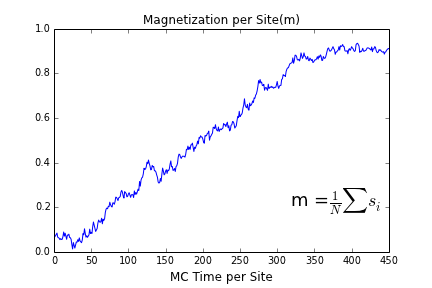
\includegraphics[width=90mm]
{../programs/graphics/equilibration_time/magnet_random_T2,000000.png}
\caption{Magnetization per Site vs MC Time per Site when T = 2.0}
\end{figure}

\newpage
\item Initial spins are all-up, corresponds to T=$0$

\begin{figure}[ht!]
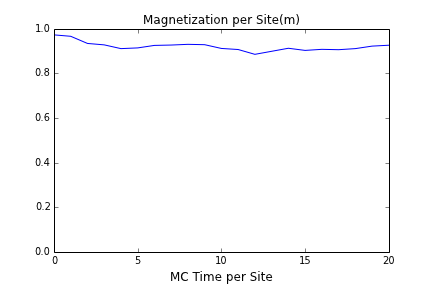
\includegraphics[width=90mm]
{../programs/graphics/equilibration_time/magnet_allup_T2,000000.png}
\caption{Magnetization per Site vs MC Time per Site when T = 2.0}
\end{figure}

\end{enumerate}

Our system's temperature is 2.0. If we start simulation with all spins to be 
random, which corresponds to T=$\infty$ case, then, we will reach 
equilibrium after about 350 MC Time per site. Also, if we start simulation 
with all up spins, which corresponds to T=0 case, then, we will get 
equilibrium about 20 MC Time per site. Therefore, we can see that if our 
initial temperature, that we start the simulation, is close to our system's 
temperature we will get equilibrium faster.

We want to analyze Ising Model for a lot of temperatures; hence, starting 
simulation with spin configuration at the end of the simulation for previous 
temperature, will decrease our equilibration time. If we are sure about that 
equilibrium is achieved, then we can analyze Ising model properties.

\subsection{Autocorrelation Function and Correlation times}

Now, we have to take independent samples from the properties after 
equilibrium is achieved. Thus, in the simulation, autocorrelation of 
quantities should be examined in the equilibrium state. Using fft() and ifft() 
functions in the program, autocorrelation function $\chi (t)$ after 
equilibrium is calculated. Autocorrelation function is proportional to 
$e^{\frac{-t}{\tau}}$ at early time steps, so, if $\chi (t)$ is normalized with 
$\chi (0)$, then $\frac{\chi (t)}{\chi (0)} = e^{\frac{-t}{\tau}}$. Now, with 
fitting this normalized autocorrelation function at early time steps with an 
exponential curve, autocorrelation time can be calculated. Taking logarithm 
of both sides, then $log(\frac{\chi (t)}{\chi (0)}) = -t/ \tau$ then $\tau = 
\frac{-1}{slope}$. Also, as mentioned before, we should take a sample 
every $2 \tau$. 

In the simulation, we consider properties magnetization per site, energy 
per site and squares of them. Hence, we will evaluate autocorrelation for 
these 4 properties and we will find 4 correlation times and we will use 
maximum of correlation times. 

Let's plot autocorrelation function with respect to MC time per Site: 

\begin{figure}[ht!]
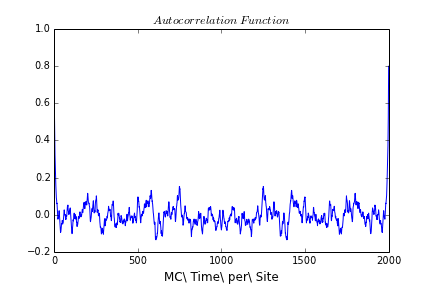
\includegraphics[width=86mm]
{../programs/graphics/autocorrelation/autocorrelation_T2,000000.png}
\caption{Autocorrelation function vs MC Time per Site when T = 2.0}
\end{figure}

\begin{figure}[ht!]
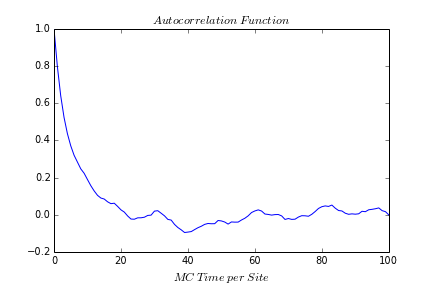
\includegraphics[width=86mm]
{../programs/graphics/autocorrelation/autocorrelation2_T2,000000.png}
\caption{Autocorrelation function vs MC Time per Site when T = 2.0}
\end{figure}

\begin{figure}[ht!]
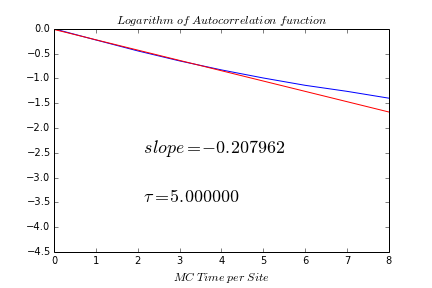
\includegraphics[width=86mm]
{../programs/graphics/autocorrelation/correlation_fit_T2,000000.png}
\caption{$log(\frac{\chi (t)}{\chi (0)})$ vs MC Time per Site when T = 2.0}
\end{figure}
\newpage
At T=2.0, we have found correlation time $\tau = 5$ [time per site] by 
fitting normalizing autocorrelation function with an exponential. 
Hence, by taking a sample in each $2 \tau$ time per site, we have 
independent data for energy and magnetization and squares of them after 
reaching the equilibrium. Also, correlation time should be maximum of 
correlation times which are found by considering magnetization, energy 
and squares of them.

\subsection{Analysis of Macroscopic System Properties}


Now, we have independent samples for energy and magnetization and 
squares of them. As previously mentioned, using these independent 
samples, we can calculate their mean values. Also, after finding mean 
values, we should calculate error estimates in them. 

With using these mean values, we can calculate magnetic susceptibility and 
specific heat, which are fluctuations in magnetization and energy.

As we defined, 
\begin{equation}
c = k J^2 N [ \langle E_{ps}^2 \rangle - \langle E_{ps} \rangle^2 ]
\end{equation}
where $E_{ps}$ is energy per site.

\begin{equation}
\chi = J N [ \langle m^2 \rangle - \langle m \rangle^2    ]
\end{equation}
We embed k in T, so in our simulation k = 1 and $J = \frac{1}{T}$. Also, to
get a complete analysis we should also add error bars to these properties. 
We can observe dependence of specific heat per site, magnetic 
susceptibility per site, internal energy per site and mean magnetization per 
site, correlation time, equilibraiton time and acceptance ratio to the 
temperature.

First, lets look at mean magnetization per site vs temperature plot:

\begin{figure}[ht!]
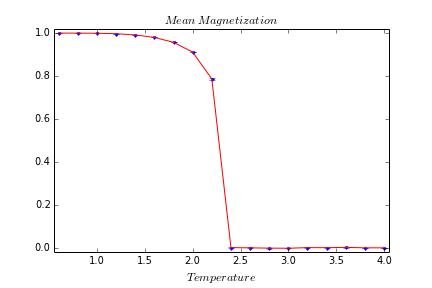
\includegraphics[width=100mm]
{../programs/graphics/properties/magnetization_L50.png}
\caption{Mean magnetization vs Temperature}
\end{figure}
If we look at the plot, mean magnetization is 1 when T=0 and 0 when 
T=$\infty$ as we expected. Also, if we increase the temperature from 0, we 
see that magnetization is about 1 until T is around 2.2. Also, if we keep on 
increasing the temperature, we will see a sharp decrease in magnetization 
to 0. This sharp change around when T is around 2.2 is called \textit{Phase 
Transition}. There is a lot of properties that should be examined at the 
phase transition. These are studied in the next section.






(YENİ)

Actually, when we reach phase transition, we expect a sharp decrease in 
magnetization, but because of finite size system, we see roundings around 
phase transition. Also, because of same reason, we see that magnetization 
after phase transition is never exactly zero, there is some deviations from 
zero.

(SON)






We can also look to internal energy of system to see the phase transition: 

\begin{figure}[ht!]
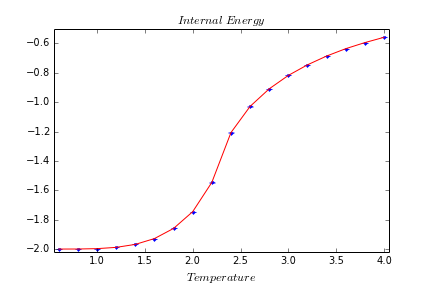
\includegraphics[width=100mm]
{../programs/graphics/properties/internal_energy_L50.png}
\caption{Internal energy vs Temperature}
\end{figure}
Again, we see that a change in internal energy of the system when T is 
around 2.2. This is also caused by phase transition.

Let's look at fluctuations in magnetization and energy, which are magnetic 
susceptibility and specific heat of the system.

\begin{figure}[ht!]
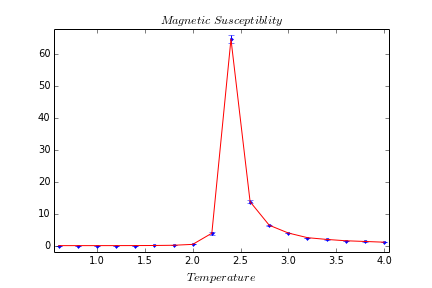
\includegraphics[width=100mm]
{../programs/graphics/properties/magnetic_suscept_L50.png}
\caption{Magnetic susceptibility vs Temperature}
\end{figure}
We can see that fluctuations in the magnetization is diverged at the 
temperature of phase transition. Hence, we see a peak at that temperature. 
Also, because of this increased fluctuations at the phase transition and 
increased correlation times at phase transition our error bars are increased. 
If we look at fluctuations in the energy;

\begin{figure}[ht!]
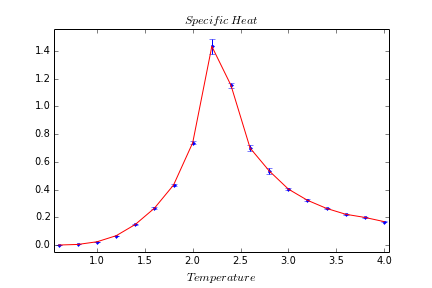
\includegraphics[width=100mm]
{../programs/graphics/properties/specific_heat_L50.png}
\caption{Specific heat vs Temperature}
\end{figure}
Fluctuations (hence, specific heat) is increased at the phase transition. 

Now look at how correlation time acts at the phase transition.

\begin{figure}[ht!]
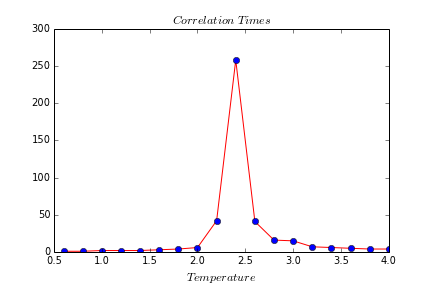
\includegraphics[width=100mm]
{../programs/graphics/properties/correlation_time_L50.png}
\caption{Correlation time vs Temperature}
\end{figure}
When phase transition occurs, our correlation times, states times between 
independent states, are diverged. Hence, because of that it is hard to 
simulate system around phase transition. Because, to get a lot of 
independent samples, we have to wait for a long time. Also, these increase 
in correlation time causes us to get a small number of samples; hence, 
causes increased error bars at the phase transition.

Also, we can look at how many attempts to flip a spin is accepted in the 
simulation, this is acceptance ratio.

\begin{figure}[ht!]
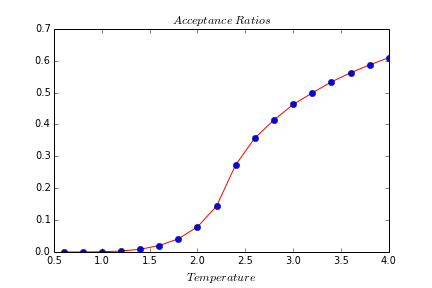
\includegraphics[width=100mm]
{../programs/graphics/properties/acceptance_ratio_L50.png}
\caption{Acceptance ratio vs Temperature}
\end{figure}
We can see that our acceptance ratio is increasing with temperature. Our 
probability to flip a spin in Metropolis simulation of Ising model is depends 
on energy difference between states. If our new state's energy is lower than 
previous state's energy, we always accept flipping. However, if it is greater, 
we accept it with a probabilty proportional to energy difference between 
states. We know that at low temperatures spins are tend to same direction, 
hence, a states of low temperature energy of system is so low and if we flip 
a spin, we generally increase the energy of the system, because to flip a 
spin we have to break to bonds between same oriented spins. Hence, it is 
hard to flip a spin at low temperatures. If we look at high temperatures, 
spin are like randomly oriented, hence energy of the system is low. Thus, 
to flip a spin we have to broke less bonds, so, flipping a spin is more likely 
to occur. 

\section{Phase Transitions}

We have seen that at phase transition, our correlation times diverge, there 
is a sharp change in magnetization and energy, hence there is a divergence 
in the magnetic susceptibility and specific heat at the phase transition. This 
phase transition is a property of the Ising model. The change occurs at 
\textit{Critical temperature}, $T_c$. For 2D Ising model, 
\begin{equation}
T_c \approx 2.269J
\end{equation}
in our case J is 1. Above critical temperature all spins are tend to random 
direction hence this phase is called \textit{paramagnetic phase}, also below 
critical temperature all spins line up in the same direction thus this phase 
is called \textit{ferromagnetic phase}. 

Now, suppose we are at high temperatures where spins are random and 
uncorrelated. If we decrease temperature, interaction between spins forces 
spins to be in same direction. Hence, spins become correlated. Spin groups 
which are correlated because of these effect are called clusters and size of 
clusters are $\xi$, correlation length. This is because of the nature of the 
Ising model. Hence, at the phase transition, we have a lot of spin groups, 
seperately. If we continue to decrease temperature, spins chose a direction 
and generate non-zero magnetization. When T goes to 0 ,  the most of the 
spins are in same direction and absolute magnetization per spin goes to 1. 

Events that occur in the critical region are called critical phenomena. We 
know that when temperature is high our spins are random when we are 
approach critical temperature from there, clusters occur, clusters includes 
spins that are correlated. Hence, when we flip a spin at critical temperature, 
these clusters flip, because spins inside it are correlated, hence, we see 
fluctuations in magnetization and energy, these fluctuations are called 
critical fluctuations. Thus, when we are approaching critical temperature 
from a high temperature, $\xi$ increases and fluctuations increase, hence 
magnetic susceptibility and specific heat increases. One of the error 
sources in critical region is these fluctuations. Actually, in thermodynamic 
limit these fluctuations diverge, but in our case, where finite size exists, 
fluctuations become very large. Hence, errors increase. The other source of 
error is correlation time. At critical temperature, most of the spins are 
correlated to each other and with Metropolis algorithm we flip spins one by 
one. Hence, to get a state which is independent of current state, we have to 
wait a long correlation time. These long correlation time causes errors in 
calculation since we need a lot of independent measurements in simulation 
and when correlation times increase, we get lower measurements and 
because of that, error becomes higher. Actually, in thermodynamical limit 
correlation time diverges at phase transition, but in our case, where finite 
size exists, correlation time becomes very high. This increase in correlation 
time is called \textit{Critical slowing down}. 

(YENI)

Also, to see critical slowing 
down, we can look at logarithm of autocorrelation function with respect to 
MC step per site.


\begin{figure}[ht!]
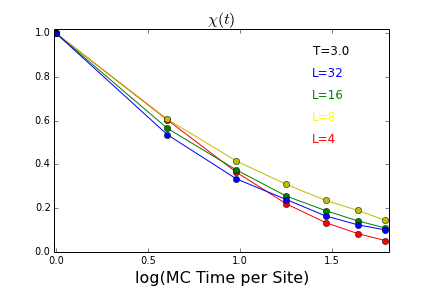
\includegraphics[width=100mm]
{../programs/graphics/properties/critical_slowing_metropolis_logtime_T=3.png}
\caption{Autocorrelation function for magnetization at T=3.0}
\end{figure}


\begin{figure}[ht!]
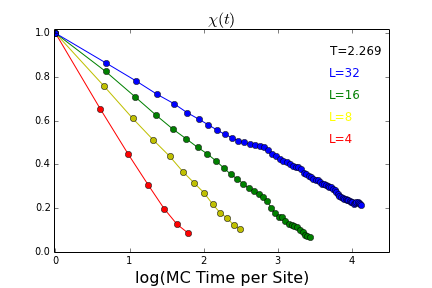
\includegraphics[width=100mm]
{../programs/graphics/properties/critical_slowing_metropolis_logtime_T=2,269.png}
\caption{Autocorrelation function for magnetization at 
T=2.269}
\end{figure}

Here, we can see that when T=3, correlation time, $\tau=-1/slope$, 
converges although we increase system size, in former figure. Also, at 
critical temperature, T=2.269, correlation time increases with system size, 
in latter figure. Hence, we can see that critical slowing down occurs when 
we increase system size.


This error source, critical slowing down, is depend on our algorithm 
whereas and fluctuation is a 
property of system. Hence, we can find a way to decrease correlation times, 
to get rid of critical slowing down,	
to increase accuracy. 

(SON)




\section{Critical and Dynamic Exponent}


( YENI EKLENDI)


Let's look at how correlation length is defined.  Spin-spin correlation 
function is 
\begin{equation}
C(\vec{r_j} -\vec{r_i}) = \langle \sigma_i \sigma_j \rangle - \langle 
\sigma_i \rangle^2
\end{equation}

According to the Ornstein-Zernicke form for long seperations of spins 
\begin{equation}
C(\vec{r})  \propto \frac{e^{-r/ \xi }}{r^{(d-2)/2}}
\end{equation}
This equation is valid for only long seperations, $r >> \xi $. 

(SON)








Also, we know that when we approach to phase transition correlation 
length increases. To measure our distance from phase transition, let us 
define reduced temperature, t.

\begin{equation}
t = \frac{|T- T_c|}{T_c}
\end{equation}

For Ising model, in thermodynamic limit, divergence of correlation length 
near phase transition then goes like 
\begin{equation}
\xi \propto t^{-\nu}
\end{equation}
\cite[p.  88]{newman} $\nu$ is critical exponent and is a property of Ising 
model, independent of J or lattice size, algorithm, ... . This is known as 
\textit{universality}. Hence, $\xi$ depends only on nature of Ising model. 







(YENI)

In thermodynamic limit, $\xi$ diverges when we approach to critical 
temperature. Hence, at critical temperature $\xi  > r$. In this case spin-
spin correlation function decays as a power law:
\begin{equation}
C(\vec{r}) = \frac{1}{r^{d-2+ \eta }}
\end{equation}
Again, $\eta$ is a  critical exponent.


(SON)






As a result of divergence of correlation length, we get divergences in 
magnetic susceptibility and specific heat in thermodynamic limit. To 
describe these divergences around phase transition, we have also 2 
universal critical exponents, 
\begin{equation}
\chi \propto t^{-\gamma}
\end{equation}
\begin{equation}
c \propto t^{-\alpha}
\end{equation}






(YENI)

We can see that, $\chi$ and c diverge at critical temperature.

Also, in thermodynamic limit, if we look at magnetization, then after the 
critical temperature it is 0 also when $T < T_c$ and $T$ is close to $T_c$;
\begin{equation}
\langle m \rangle \propto (T_c - T )^\beta
\end{equation}
Again, $\beta$ is a critical exponent


These critical exponents depends our system, independent of our 
algorithm and fall into \textit{universality classes}. Also, these critical 
exponents depends on each other and values of these expoenents can be 
found for the 2D Ising Model with considering renormalization group 
theory.

(SON)






Also, we can describe divergence in correlation time per site
\begin{equation}
\tau \propto t^{-z \nu}
\end{equation}
where z is dynamic exponent.

Hence, with using dynamic exponent, we can analyze critical slowing down 
effect. Also, we know that critical slowing down depends on our algorithm. 
Hence, z depends on our algorithm, then, we want small z values in our 
algorithm. If z = 0, there is no critical slowing down and we can simulate 
Ising model around phase transition, efficiently. 






(YENI)

For the 2D Ising Model we know critical temperature. If we know critical 
temperature analitically, to measure critical exponents and dynamic 
exponent, 
we can look at finite size scaling. Also, with using finite size scaling we can 
find critical temperature. 


\section{Measurement of Dynamic Exponent, z}

(SON)






Let's find dynamic exponents z for the Metropolis algorithm with finite size 
scaling. 

Now, we know that 
\begin{equation}
\tau \propto \xi^{z}
\end{equation}
we know that $\xi$ diverges near phase transition; hence, correlation times 
near phase transition are getting bigger.  

In Monte Carlo simulations, we simulate models within a finite size. 
Because of finite size, correlation times actually can never really diverge. 
In a simulation, maximum value of correlation length is $L^d$, where $d$ 
is 
dimension of our system. Therefore, when we are at critical temperature, 
our correlation length is approximatelly $L^2$ for an 2D Ising model.
\begin{equation}
\tau \propto L^{z}
\end{equation} 

At $T=T_c$, if we plot correlation times with respect to L on logarithmic 
scale, we can get z. 

For Metropolis Algorithm: 
\begin{figure}[ht!]
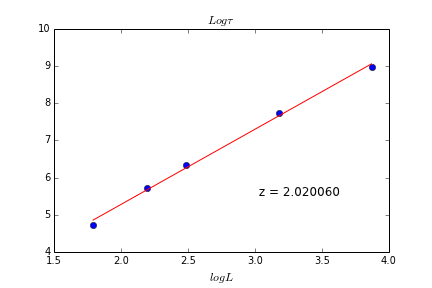
\includegraphics[width=100mm]
{../programs/graphics/properties/dynamic_exponent.png}
\caption{$log\tau$ vs $logL$}
\end{figure}
z is found as 2.02. This z is a high value for Monte Carlo simulations. 
Hence, it causes a great critical slowing down. Now, with using different 
algorithms we want to decrease dynamic exponent values, hence, want to 
decrease correlation times. If we look at Wolff algorithm, we get a lower 
value of z, hence, we expect that Wolff algorithm is better than Metropolis 
algorithm near phase transition. When, we are away from critical 
temperature ($T_c$) Metropolis algorithm is a good choice to simulate 
Ising model. 
When we approach to $T_c$, correlation times are getting bigger and it 
makes hard 
to get sufficient independent values.  Hence, because of this effect errors 
increase when we approach the phase transition. 

\section{Wolff Algorithm}

Correlation times increase with $L^z$ at critical temperature. CPU time to 
perform Monte Carlo steps per site increase with $L^d$ because we have 
$L^d$ sites. Hence, CPU time to simulate one correlation time for 2D Ising 
model is
\begin{equation}
\tau_{CPU} \propto L^{2+z}
\end{equation}
Also, we found z is around 2, hence $\tau_{CPU} \propto L^{4}$ . This is a 
big time for simulating the system around critical temperature. 

The reason of that z is high values in Metropolis algorithm is because of 
divergence of correlation length $\xi$ and critical fluctations near phase 
transition. When T is closer to critical temperature, correlation length is 
getting bigger and large regions of spins are in same direction. This 
regions are called domains. When $T = T_c$ , $J = 0.44 $ ; hence, $T_c = 
2,269 J $, $A(\mu \rightarrow \nu) \approx e^{-8J/T_c} \approx 0.03 $ 
This is about $ 3 \% $ to flip a spin inside a domain. Therefore, for  
Metropolis algorithm it is difficult to flip a spin because it tries to flip spin 
by spin. As a result of this, acceptance ratio is very low around critical 
temperature and generally, we don't change state. Because of this, 
simulation time diverges around critical temperature.

Also, chance of flip a spin at the edge of a domain is high because it has 
opposite spins in its neighbourhood, hence lower energy cost. The basic 
idea of Wolff algorithm is to look for clusters of similarly oriented spins and 
then flip them in their entirely all in one go, rather than trying to turn them 
over spin by spin.\cite[p. 92]{newman}
These algorithms that flips clusters are called Cluster-Flipping algorithms 
or simply Cluster algorithms.  With using Cluster algorithms we can get rid 
of critical slowing down. 

To find clusters, a spin is picked at random and we look at the 
neighbourhood of this spin to find a spin in same direction. If we find a 
spin in same direction, then we use the same procedure for this spin. By 
iterating in this way, we can form cluster. We don't want to flip all 
neighbouring spins in same direction, hence, this flipping a spin depends 
on temperature. If T is high, spins are generally uncorrelated and we want 
to flip little clusters. When T is around critical temperature, cluster size 
increases. When T is lower than critical temperature, ferromagnetism come 
in action and most of the spins in same direction, like one cluster. Hence, 
we understand that if T decreases, cluster size to flip increases. Because of 
this, we add a spin to cluster to flip it with a probability $P_{add}$ and we 
expect that $P_{add}$ is negatively proportional to the temperature.


After sweeping the lattice and adding spins to cluster with a probability, we 
flip the cluster with an acceptance ratio which depends on energy cost to 
flip cluster.

With choosing these probabilities, we want to satisfy detailed balance for a 
given $P_{add}$ and we want acceptance ratio as close to 1 by choosing 
$P_{add}$.

Suppose that we have chosen a cluster in state $\mu$ and with flipping 
these spins in cluster, we went to the state $\nu$. If there is a spin 
neighbouring to the cluster, to flip the cluster we have to break these 
bonds. Let's create the cluster with choosing a random spin and adding 
spins to cluster in the same direction with $P_{add}$. Also, suppose we 
have rejected m spins to add to cluster with $1- P_{add}$; hence, there are 
m bonds to broke. Hence, selection probability $g(\mu \rightarrow \nu) = 
1-P_{add}^m$. Also, suppose that for the same cluster there are n bounds 
to broke for a reverse move, $\nu \rightarrow \mu$. Thus, $g(\nu 
\rightarrow \mu) = 1-P_{add}^n$
To satisfy detailed balance,
\begin{equation}
\frac{P(\mu \rightarrow \nu) }{P(\nu \rightarrow \mu) } = \frac{g(\mu 
\rightarrow \nu)A(\mu \rightarrow \nu)  }{g(\nu \rightarrow \mu) A(\nu 
\rightarrow \mu) } = \frac{P_\nu}{P_\mu} = e^{-\beta(E_\nu - E_\mu)} = 
(1- P_{add})^{m-n} \frac{A(\mu \rightarrow \nu) }{A(\nu \rightarrow \mu) }
\end{equation}

$E_\nu $ and $E_\mu$ depends on bonds will broken. To break m bonds 
we need energy $m2J$ and to make n bonds we need energy $-n2J$. 

\begin{equation}
E_\nu - E_\mu = 2J(m-n)
\end{equation}
Hence,
\begin{equation}
\frac{A(\mu \rightarrow \nu)}{A(\nu \rightarrow \mu) } = ((1- 
P_{add})e^{\beta 2J})^{n-m}  
\end{equation}

If we choose $P_{add} = 1 - e^{-2\beta J}$, then acceptance ratios are 
equal and independent of anything. With choosing acceptance ratios as 1 
and $P_{add} = 1 - e^{-2 \beta J}$, we will satisfy detailed balance 
condition and accept to flip the cluster always. 

Also, ergodicity conditions is satisfied. We have always a chance to accept a 
neighboring spin to the cluster and flipping the cluster we get a new state. 
Hence, we have always a probability to access a state. 

$P_{add}$ is inversely proportional to temperature. When T=0, $P_{add}$  
is 1 and when $T=\infty$, $P_{add}$  is 0. This means that size of cluster 
is inversely proportional to temperature.  

\section{Implementation of Wolff simulation of the Ising Model}



After, defining initial properties we can start the simulation. Simulation 
goes like this: 

\begin{enumerate}
\item Select a spin randomly.
\item Look at the neighboring spins. If they are in same direction, add the 
cluster with probability $P_{add}$
\item For a spin that is added to the cluster, look at the neighboring spins 
of this spin and again add the spins with same direction which are not in 
the cluster with probability $P_{add}$
\item Repeat the process and complete the cluster
\item Flip the cluster
\end{enumerate}
This is the Wolff simulation of the Ising Model. 

Now, we expect that correlation times to decrease when Wolff algorithm is 
used. To see, it we can compare dynamic exponents of Wolff algorithm and 
Metropolis algorithm. 



In Wolff algorithm we flip spins in a cluster. If there is n spins in a cluster, 
we flip n spins. Also, in Metropolis algorithm we flip 1 spin. Hence, to make 
a fair description of correlation time, this difference must be considered. 
We calculated correlation times for Metropolis algorithm in MC time per 
site. Thus, to achieve an independent state, we have to wait $\tau$ trials of 
flipping 1 spin, per spin, in scrictly speaking. Also, again if we calculate 
correlation times for Wolff algorithm as in Metropolis algorithm, again we 
have to wait $\frac{\tau}{\langle n \rangle / L^d } $ trials of flipping 1 spin, 
per spin. Hence, if we multiply which is found in Wolff algorithm with 
$\frac{\langle n \rangle }{L^d} $, we make a fair calculation of correlation 
time. Therefore,
\begin{equation}
\tau = \tau_{steps} \frac{\langle n \rangle }{L^d}
\end{equation}
Where $\tau_{steps}$ is found in Wolff algorithm and $\langle n \rangle$ is 
mean value of cluster sizes. 
\newpage
For Wolff Algorithm: 
\begin{figure}[ht!]
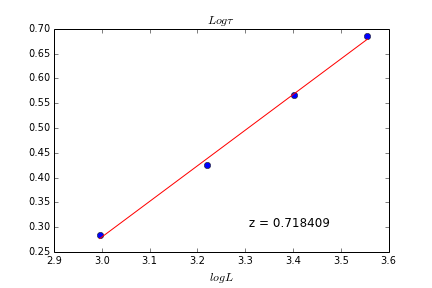
\includegraphics[width=100mm]
{../programs/graphics/properties/dynamic_exponent_wolff.png}
\caption{$log\tau$ vs $logL$}
\end{figure}

Now, we can compare Wolff and Metropolis algorithms in the critical 
region. If we look at dynamic exponent values for two algorithms, then we 
can see that, for Metropolis algorithm $z=2.02$ and for Wolff algorithm 
$z=0.72$. We know that $\tau \propto L^{z}$ at critical temperature for a 
finite size system. Hence, we can see that at critical temperature Wolff 
algorithm's correlation time is much lower than Metropolis algorithm's. 
Also, CPU time to simulate one correlation time for 2D Ising model is 
$\tau_{CPU} \propto L^{2+z} $, hence, CPU time is, also, much lower for 
Wolff algorithm. Besides, we can compare correlation times that we found 
for two algorithms. For instance, for a 20x20 lattice, with Metropolis 
algorithm $\tau=1040 $ MC step per site and with Wolff algorithm $\tau= 
4 $ MC step per site, at critical temperature. There is a huge difference in 
correlation time values for two algorithms. 

If we want to analyze behaviour of the model at $T_c$, a cluster spin 
algorithm, such as Wolff algorithm, is more efficient than a single spin 
algorithm, such as Metropolis algorithm. 



\chapter{Finite Size Scaling}

We have look at finite size scaling method to find dynamic exponent, z, to 
investigate our algorithm's efficiency. To find critical temperature and 
critical exponents, which are found analitically for 2D Ising model,  we 
should also look at finite size scaling. For the 2D Ising Model, $T_c = 
\frac{2}{ln(1+ \sqrt{2})} \approx 2.269 \quad \nu = 1 \quad \beta = 
\frac{1}{8} \quad
\gamma= \frac{7}{4} \quad \alpha=0$

We know that correlation length diverges in thermodynamic limit at critical 
temperature, but in 
our case of finite size system, maximum value of correlation length is 
$L$, which is system size. Because of this cut-off in correlation length, 
other divergent quantities, like magnetic susceptibility and specific heat, 
will cut-off when $\xi = L$. As explained before, another effect of finite 
size system is rounding of magnetization around critical temperature. This 
region is in which infinite-size correlation length exceeds L.\cite{sandvik}

Now, we want to find critical exponents with using finite size scaling. 
We will see that, for a $t \neq 0$, at a system size 
$L \approx \xi (t) $  and our expectations of properties converge to 
thermodynamic values at this t. Hence, with using this, we can calculate 
critical exponents.

Let a property $Q \propto t^{-\lambda}$ in thermodynamic limit, we 
expect that property Q to be diverge at critical temperature. But, because 
of finite size system, we see an increase in property Q at a $t \neq 0$.
To find $\lambda$, $lnA = c - \lambda lnt$ 
where c is a constant. We know what critical temperature is, hence if we 
plot lnA versus lnt, we can estimate $\lambda$ with a linear fit. Also, if we 
don't know what $T_c$ is, with changing $T_c$, we can look for where best 
linear fit occurs. But, we know that we see that an increase in quantity Q at 
$t \neq 0 $, hence, to get a good estimate of $T_c$ and critical exponents, 
we have to go to very 
large systems, this will be explained later. Also, we have to reach very large 
systems, because our 
peak is cut off because of finite size system. There is a big effect of system 
size on critical exponents and critical temperature, in this case. 

Now, we know how to analyze a property which diverges at critical 
temperature in thermodynamic limit. Let's, look at a property which is in 
different form, magnetization. $\langle m \rangle  \propto (T_c - 
T)^\beta$ when $T < T_c$. Again, taking logarithm of both sides 
$$ln \langle m \rangle = c + \beta ln(T_c-T)$$ Again, with using linearity 
between $\langle m \rangle$ and $T_c - T$, we can calculate $\beta$.

If we plot it, we can see that when $T_c - T < A$, linearity is more 
accurate. Also, if T is so close to $T_c$, rounding sets in because of finite 
size system and 
linearity is spoiled.  Again, we expect a better approximation to $\beta$ in 
thermodynamic limit if we increase L, because in this case rounding area is 
smaller, but still exists.  



Plotting quantity with respect to a function of temperature, gives 
us a straight forward method to calculate critical exponents and critical 
temperature. In this case, to overcome finite size system deviations, we 
have to go to very large systems. Also, to get critical exponents and critical 
temperature, we can use regularity in these deviations in a finite size 
scaling. The basis of finite size scaling is that deviations from the infinite 
size critical behaviour occurs when correlation length $\xi $ becomes 
comparable with system length L. \cite{sandvik}

We know that, $\xi \propto t^{-\nu}$, we can write it as $t \propto 
\xi^{-1/\nu}$. Also, $\chi \propto t^{-\gamma}$, then $\chi \propto 
\xi^{\gamma / \nu}$. At a reduced temperature, $t \neq 0$, $L \approx 
\xi$ and 
$$\chi (L) \propto L^{\gamma / \nu}$$
Also, at a reduced temperature, $t \neq 0$, $$t(L) \propto L^{-1/\nu}$$ 
Here, we can see that if we increase L, we will see these critical phenomena 
close to critical temperature in thermodynamic limit, if $\nu$ is a positive 
number, which is in the 2D Ising Model. For example, 
we see maximum of magnetic susceptibility at $t(L)$ and its value is $\chi 
(L)$.

\begin{figure}[ht!]
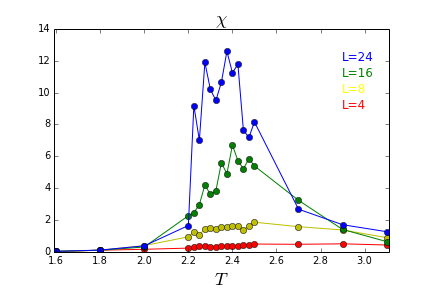
\includegraphics[width=100mm]
{../programs/graphics/properties/magnetic_suscept_wolff.png}
\caption{Magnetic Susceptibility vs Temperature}
\end{figure}


\newpage
We can see that, peak of magnetic susceptibility is increased with L, as 
expected, hence because of that we expect $\frac{\gamma}{\nu} > 0$. 
Also, by increasing L, position of peak of magnetic susceptibility 
approaches to critical 
temperature in thermodynamic limit, $T_c = 2.269$, thus $\nu>0$.

Now, with using these equations we want to extract critical temperature 
and critical exponents. If we take logarithm of both sides of equation of 
maximum values of
magnetic susceptibility, which occurs at $L \approx \xi$, $ln \chi (L) = a + 
\frac{\gamma}{\nu} lnL$, where a 
is a constant, hence 
with a linear fit to these peak values of magnetic susceptibility, we can find 
$\frac{\gamma}{\nu}$


\begin{figure}[ht!]
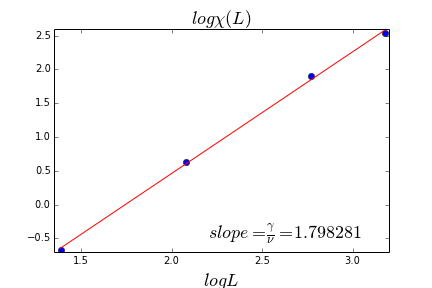
\includegraphics[width=100mm]
{../programs/graphics/properties/gamma_over_nu_wolff.png}
\caption{$\gamma / \nu$}
\end{figure}

Here, we found $\frac{\gamma}{\nu}=1.798$, also, we expect it to find 
$\frac{\gamma}{\nu}=\frac{7}{4}=1.750$. It is a good approximation for 
ratios of these critical exponents.

Also, if we take logarithm of reduced temperature equation $ln t(L) = b + 
\frac{-1}{\nu} lnL$, where b is a constant, then with a linear fit, we can find 
$\nu$, if we know critical temperature. Also if we want to find $T_c$, then 
by adjusting $T_c$ to get a 
linear behavior between $ln t(L)$ and $lnL$, we can find $T_c$ and with 
using this $T_c$, we can find $\nu$. 

We know $T_c=2.269$, with using this critical temperature value,

\begin{figure}[ht!]
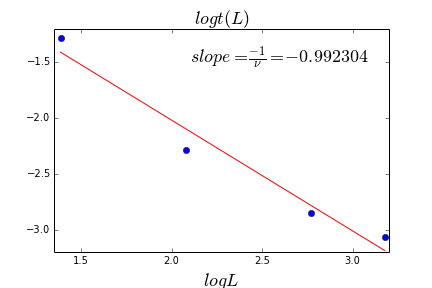
\includegraphics[width=100mm]
{../programs/graphics/properties/one_over_nu_wolff.png}
\caption{$1 / \nu$}
\end{figure}

We found $\nu = -1 / (slope) = 1.008$. Hence, $\gamma=1.812$, where 
$\nu = 1$ and $\gamma=1.750$ theoretically.

This finite-scaling procedure (for properties diverges at critical 
temperature) obeys a more general \textit{finite size 
scaling hypothesis}. The hypothesis is when temperature is close to critical 
temperature, observable is equal to a power of L multiplied by a non 
divergent function 
$\xi / L$. \cite{sandvik}. Hence, for magnetic susceptibility, 
\begin{equation}
\chi (t,L) = L^\sigma f(\xi / L)
\end{equation}
by using $ \xi \propto t^{-1 / \nu}$, we get
\begin{equation}
\chi (t,L) = L^\sigma g(tL^{1/ \nu})
\end{equation}  




/////

NOT:

BURAYI ANLAMADIM NOTLARDAN. $\xi \propto t^{-\nu}$ degil miydi ? 
Eqn, 80 den 81 e nasıl geçildi?????


/////


where, $g(tL^{1/ \nu})$ is a scaling function. 

We know that in thermodynamic 
limit ($L \rightarrow \infty $) when t is close to 0, $\chi \propto 
t^{-\gamma} $. To satisfy this form, 
$g(x) \propto x^{-\gamma}$ for $x \rightarrow \infty $ and $\sigma = 
\frac{\gamma}{\nu}$.
Hence finite size scaling form is,
\begin{equation}
\chi (t,L) = L^{\gamma / \nu } g(tL^{1/\nu})
\end{equation}

To extract scaling function, we can plot $\frac{\chi}{L^{\gamma / \nu}}$ 
with respect 
to $x= tL^{1/\nu}$ for different system sizes. In each plot, we expect to 
find a similar curve, which is scaling function, for large system sizes.

\begin{figure}[ht!]
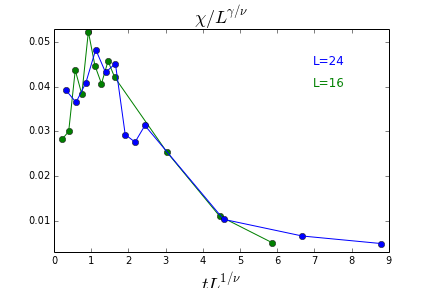
\includegraphics[width=100mm]
{../programs/graphics/properties/scaled_magnetic_suscept_wolff.png}
\caption{Finite size scaling}
\end{figure}

These curves are similar to each other, if we make a simulation for larger 
system sizes and with using more datas in our calculations, we will get 
more similar curves.

We know that, maximum values of magnetic susceptibility $\chi (L) 
\propto L^{\gamma / nu}$, hence because of our scaling in the y axis, we 
see that peaks are in same magnitude in y axis. Also, reduced 
temperatures where these peaks occur are $t(L) \propto L^{-1/ \nu}$, 
therefore because of our scaling in the x axis, we that peaks in same x 
coordinates.

To extract critical temperature and $\gamma / \nu $, we can adjust critical 
temperature 
and critical exponents, until curves coincide. 

////

NOT: 

curverler cakısana kadar exponentlar degistirilerek mi exponent degerleri 
elde edilecek. Tam olarak nasıl bulacagımızı anlamadım bu yontem ile ?

////



In this case, we will find same critical exponents values as before, we only 
described a new scaling procedure to find 
them.


Also, in particular, to extract critical temperature and $\gamma / \nu $, 
scaling exactly at 
critical temperature can be used:
\begin{equation}
\chi (T_c, L ) \propto L^{\gamma / \nu}
\end{equation}
with using linear fit to find critical temperature and critical 
exponents as before, we can find them. 


Let's look at finite size scaling for specific heat: 
For specific heat finite size form should be 
\begin{equation}
c(t,L) = L^{\alpha / \nu} g(tL^{1 / \nu})
\end{equation}

We know that for the 2D Ising Model, $\alpha=0$. Hence, $c/ L^{\alpha / 
\nu} = c$. If we plot c with respect to $x=tL^{1 / \nu}$:

\begin{figure}[ht!]
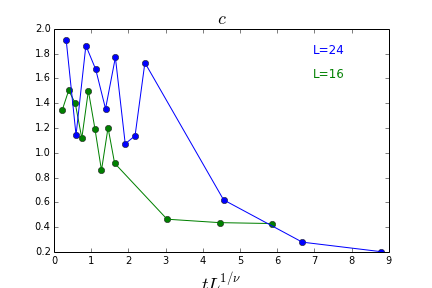
\includegraphics[width=100mm]
{../programs/graphics/properties/scaled_spec_heat_wolff.png}
\caption{Finite size scaling}
\end{figure}

Curves are not same in this case, so it means that our equation for specific 
heat finite size form is not valid. This is understood as being due to a 
logarithmic scaling when $\alpha = 0 $ i.e.,
\begin{equation}
c(t,L) = ln(L) g(tL^{1 / \nu})
\end{equation}
\cite{sandvik}

Again, if we plot $c / lnL$ with respect to $x=tL^{1 / \nu}$:

\begin{figure}[ht!]
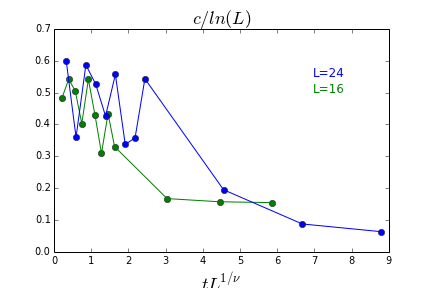
\includegraphics[width=100mm]
{../programs/graphics/properties/scaled_log_spec_heat_wolff.png}
\caption{Finite size scaling}
\end{figure}

Now, with using logairthmic scaling, we get similar curves. Again if 
we make a simulation for larger system sizes and with using more datas in 
our calculations, we will get 
more similar curves. This logarithmic scaling is an anomaly for the 2D Ising 
model, it is because of $\alpha = 0$


In finite size scaling, to find critical temperature and critical exponents, we 
adjust critical temperature and an exponent until curves collapse or until 
we 
see a linear function in log-log plot of a divergent quantity. This 
simultaneous adjusting of critical temperature and critical exponents is 
hard to do. This two-parameter scaling can be easily affected by 
corrections to the leading finite-size scaling forms.\cite{sandvik}
If we construct a new method to calculate critical temperature without 
using exponents, 
then by using this critical temperature, we can find critical exponents more 
easily. 



\chapter{Binder Ratios}


At critical temperature, ratio of two quantities which have same critical 
exponents, should be independent of size at critical temperature. Because, 
these critical exponents decide quantities dependence on system size. One 
of these ratios is ratios of powers of magnetization which is called 
\textit{Binder ratios}. We know that $$ \chi = \beta N (\langle m^2 \rangle 
- \langle m \rangle^2)$$, when there is no external magnetic field. Also, 
when T is greater than critical temperature, we know that $\langle m 
\rangle = 0 $, hence $$\chi = \beta N \langle m^2 \rangle $$.


NOT::::

((((((

$ \chi \approx L^{\gamma / \nu} \quad \chi \approx t^{- \gamma }  $
$\xi \approx t^{-\nu} $
kullanarak nasıl $<m^2>$ nin 
$ t^{-(\gamma / \nu - d)}  $ 
seklinde gittigini ve bunun nasıl $<m>^2$ nin girişiyle aynı oldugunu 
anlamadım.

((((((


\begin{figure}[ht!]
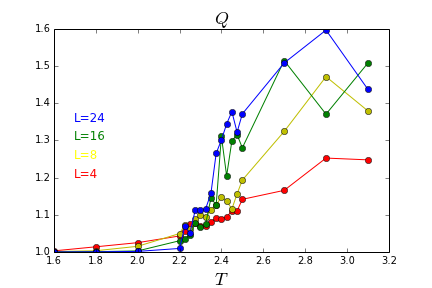
\includegraphics[width=100mm]
{../programs/graphics/properties/binder_ratio_wolff.png}
\caption{Finite size scaling}
\end{figure}



\begin{figure}[ht!]
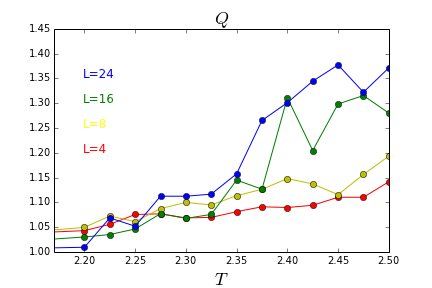
\includegraphics[width=100mm]
{../programs/graphics/properties/binder_ratio2_wolff.png}
\caption{Finite size scaling}
\end{figure}


Here, we can see that curves cross at approximately at $T=2.25$. Hence, 
$T_c = 2.25$



\chapter{Stochastic Series Expansion (SSE)}

In a Monte Carlo simulation to calculate expectation value of a quantity, 
instead of considering all states of the system, we use a portion of the 
states of the system, using importance sampling. 

For the 2D Ising model, to calculate expectation value:
$$
\langle Q \rangle = \frac{\sum\limits_{\mu} Q_\mu e^{-\beta E_\mu}}
{\sum\limits_{\mu} e^{-\beta E_\mu}}=\frac{1}{Z} \sum\limits_{\mu} 
Q_\mu e^{-\beta E_\mu}
$$
We choose a portion of the states of the system from a probability 
distribution $P_\mu$, in this case estimation of expectation value is
$$
Q_M = \frac{\sum\limits_{i=1}^M {Q_\mu}_i {{P_\mu}_i}^{-1} e^{-\beta 
{E_\mu}_i}}{\sum\limits_{j=1}^M {{P_\mu}_j}^{-1} e^{-\beta{E_\mu}_j}}
$$
Also, using importance sampling,
$$
P_\mu = Z^{-1} W_\mu
$$
$$
W_\mu = e^{-\beta E \mu} 
$$
we get
$$
Q_M = \frac{1}{M} \sum\limits_{i=1}^M {Q_\mu}_i 
$$

Besides, to create states obeying $P_\mu$, we use Markov-Chain sampling 
and to get desired probability distribution $P_\mu$, we have to satisfy 3 
conditions: 
\begin{enumerate}
\item $\frac{P(\mu \rightarrow \nu)}{P(\nu \rightarrow \mu)} = \frac{P_\nu 
}{P_\mu } $ (detailed balance)
\item $\sum\limits_{\nu} P(\mu \rightarrow \nu )  =1 $
\item Ergodicity
\end{enumerate}

Now, suppose that we cannot evaluate exponential function for $P_\mu$ 
and we can evaluate any power of a number: 
If we expand exponential function to Taylor Series, we get:
$$
e^x = \sum_{n=0}^\infty \frac{x^n}{n!}
$$
Hence, 
\begin{equation}
\langle Q \rangle =\frac{1}{Z} \sum\limits_{\mu} \sum_{n=0}^\infty 
Q_\mu \frac{(-\beta E)^n}{n!}
\end{equation}
and 
\begin{equation}
Z=\sum\limits_{\mu} \sum_{n=0}^\infty 
\frac{(-\beta E)^n}{n!}
\end{equation}

We can think of this as having enlarged our configuration space into an 
expansion dimension whose coordinate to be sampled is the expansion 
power n.\cite{sandvik_sse}
Again, using importance sampling in this enlarged space,
\begin{gather}
P_{\mu,n} = Z^{-1}W_{\mu,n} \qquad
W_{\mu,n} = \frac{(-\beta E)^n}{n!}
\end{gather}
then, we get again
\begin{equation}
Q_M = \frac{1}{M} \sum\limits_{i=1}^M {Q_{(\mu,n)}}_i 
\end{equation}
Now, we make sampling in space $\{\sigma,n\}$ configuration space. 

We expect that, probability distribution $P_\mu$ to be positive. To make 
probability distribution positive in all cases, we can substract a constant 
$\epsilon$ from energy, to make all energy values of the system negative. 
Hence, $\epsilon$ should be equal to or bigger than maximum energy 
value of the system.

Hence, our weight function is:
\begin{equation}
W_{\mu,n} = \frac{\beta^n}{n!} [\epsilon - E_\mu]^n \qquad P_{\mu,n} = 
Z^{-1}W_{\mu,n}
\end{equation}

Again, we want to create states obeying $P_{\mu,n}$. Hence, we have to 
satisfy again 3 conditions:

\begin{enumerate}
\item $\frac{P(\mu,m \rightarrow \nu,n)}{P(\nu,n \rightarrow \mu,m)} = 
\frac{P_{\nu,n} 
}{P_{\mu,m} } = \frac{\beta^n}{n!}\frac{m!}{\beta^m}\frac{[\epsilon - 
E_\nu]^n}{[\epsilon - E_\mu]^m}$ 
\item $\sum\limits_{\nu,n} P(\mu,m \rightarrow \nu,n )  =1 $
\item Ergodicity
\end{enumerate}
Also, we can write first condition in terms of selection probabilities and 
acceptance ratios. If we write it, we get
\begin{equation}
\frac{A(\mu,m \rightarrow \nu,n)}{A(\nu,n \rightarrow \mu,m)} = 
\frac{\beta^n}{n!}\frac{m!}{\beta^m}\frac{[\epsilon - E_\nu]^n}{[\epsilon - 
E_\mu]^m}
\end{equation}

Again, we can choose acceptance probabilities as:
\[
    A(\mu,m \rightarrow \nu,n)= 
\begin{cases}
    \frac{\beta^n}{n!}\frac{m!}{\beta^m}\frac{[\epsilon - E_\nu]^n}{[\epsilon 
    - 
E_\mu]^m},& \text{if } E_\nu > E_\mu\\
    1,              & \text{otherwise}
\end{cases}
\]

Let's first consider a move in expansion dimension, from m to n, in a spin 
configuration corresponding to energy $E_\mu$. Also, let possible values 
for n are m, m+1 and m-1. In this 
case 
\begin{equation}
\frac{A(m \rightarrow n)}{A(n \rightarrow m)} = 
\frac{\beta^n}{n!}\frac{m!}{\beta^m}\frac{[\epsilon - E_\mu]^n}{[\epsilon - 
E_\mu]^m}=[\beta (\epsilon - E\mu )]^{n-m} \frac{m!}{n! }
\end{equation}
(We presumed that all selection probabilities are equal between possible 
moves.)
Suppose n=m:
\begin{gather}
\frac{A(m \rightarrow n)}{A(n \rightarrow m)}  = 1  \qquad A(m \rightarrow 
n) = 1 
\end{gather}
This means that, we always accept that move from m to n. 
When n=m+1:
\begin{equation}
\frac{A(m \rightarrow n)}{A(n \rightarrow m)} = \frac{\beta (\epsilon - 
E\mu )}{m+1}
\end{equation} 
Also, when n=m-1:
\begin{equation}
\frac{A(m \rightarrow n)}{A(n \rightarrow m)} = \frac{m}{\beta (\epsilon - 
E\mu )}
\end{equation}
Hence,
\[
    A(m \rightarrow n)= 
\begin{cases}
   1 ,& \text{if } n=m\\
    1,              & \text{if } n=m+1 , \beta (\epsilon - E_\mu) \geq m+1\\
    \frac{\beta (\epsilon - E_\mu)}{m+1},  & \text{if } n = m+1 ,  \beta 
    (\epsilon - E_\mu) < m+1 \\
    1, & \text{if } n = m-1 ,  \beta (\epsilon - E_\mu) \leq m \\
    \frac{m}{\beta (\epsilon - E_\mu)}, & \text{if } n = m-1 ,  \beta (\epsilon 
    - E_\mu) > m \\
    
\end{cases}
\]

After changing the expansion dimension, we can consider a change in spin 
configuration with respect to:
\begin{equation}
\frac{A(\mu \rightarrow \nu)}{A(\nu \rightarrow \mu)} = \frac{(\epsilon - 
E_\nu)^n}{(\epsilon - E_\mu)^n}
\end{equation}
\[
    A(\mu \rightarrow \nu)= 
\begin{cases}
   \frac{(\epsilon - E_\nu)^n}{(\epsilon - E_\mu)^n} ,& \text{if } E_\nu > 
   E_\mu\\
    1,              & \text{otherwise}
\end{cases}
\]


In the simulation, firstly we try to move from expansion dimenson m to 
another dimension n. After this trial, we try to change spin configuration 
with flipping 1 spin, independent from the first trial. Hence, our probability 
to move from a configuration 
space $\{\mu, m\}$ to $\{\nu, n \}$ is 
\begin{equation}
P(\mu,m \rightarrow \nu,n) = P(\mu \rightarrow \nu) P(m \rightarrow n)
\end{equation}
Also, we defined these probabilities in terms of selection probabilities and 
acceptance ratios.
\begin{equation}
P(\mu \rightarrow \nu) P(m \rightarrow n)= 
g(\mu \rightarrow \nu) g(m \rightarrow n) A(\mu \rightarrow \nu)A(m 
\rightarrow n)
\end{equation}
We know that for the 2D Ising Model $g(\mu \rightarrow \nu)=\frac{1}{N}$, 
it means that we select new spin configurations with equal probabilities, 
by changing 1 spin in Metropolis Algorithm. Also, we are selecting new 
expansion dimensons with equal probabilities, this means that $g(m 
\rightarrow n)= \frac{1}{3}$

Besides, we can define a total selection probability and acceptance ratio for 
SSE method:
\begin{gather}
g(\mu,m \rightarrow \nu,n) = g(\mu \rightarrow \nu) g(m \rightarrow n) 
\\
A(\mu,m \rightarrow \nu,n) = A(\mu \rightarrow \nu) A(m \rightarrow n)
\\
P(\mu,m \rightarrow \nu,n) = g(\mu,m \rightarrow \nu,n) A(\mu,m 
\rightarrow \nu,n)
\end{gather}
Hence, 
\begin{equation}
g(\mu,m \rightarrow \nu,n) = \frac{1}{3N}
\end{equation}
for any move in configuration space from $\{\mu, m\}$ to $\{\nu, n\}$.
Also,
\[
    A(\mu, m \rightarrow \nu, n)= 
\begin{cases}
   \frac{(\epsilon - E_\nu)^n}{(\epsilon - E_\mu)^n} ,& \text{if } n=m, E_\nu 
   > 
   E_\mu\\
    \frac{(\epsilon - E_\nu)^n}{(\epsilon - E_\mu)^n},              & \text{if } 
    n=m+1 , 
    \beta (\epsilon - E_\mu) \geq m+1, E_\nu > E_\mu\\
    \frac{\beta (\epsilon - E_\mu)}{m+1 }\frac{(\epsilon - E_\nu)^n}
    {(\epsilon - 
    E_\mu)^n},  & \text{if } n = m+1 ,  \beta 
    (\epsilon - E_\mu) < m+1, E_\nu > E_\mu \\
    \frac{(\epsilon - E_\nu)^n}{(\epsilon - E_\mu)^n}, & \text{if } n = m-1 ,  
    \beta 
    (\epsilon - E_\mu) \leq m, E_\nu > E_\mu \\
    \frac{m}{\beta (\epsilon - E_\mu)} \frac{(\epsilon - E_\nu)^n}{(\epsilon - 
    E_\mu)^n}, & \text{if } n = m-1 ,  \beta (\epsilon 
    - E_\mu) > m, E_\nu > E_\mu \\
       1 ,& \text{if } n=m, E_\nu \leq E_\mu\\
    1,              & \text{if } n=m+1 , \beta (\epsilon - E_\mu) \geq m+1, 
    E_\nu \leq E_\mu\\
    \frac{\beta (\epsilon - E_\mu)}{m+1},  & \text{if } n = m+1 ,  \beta 
    (\epsilon - E_\mu) < m+1, E_\nu \leq E_\mu \\
    1, & \text{if } n = m-1 ,  \beta (\epsilon - E_\mu) \leq m, E_\nu \leq 
    E_\mu \\
    \frac{m}{\beta (\epsilon - E_\mu)}, & \text{if } n = m-1 ,  \beta (\epsilon 
    - E_\mu) > m, E_\nu \leq E_\mu \\
    

\end{cases}
\]
If we look at, in all cases,
\begin{equation}
\frac{P(\mu,m \rightarrow \nu,n)}{P(\nu,n \rightarrow \mu,m)} = 
\frac{P_{\nu,n} 
}{P_{\mu,m} } = \frac{\beta^n}{n!}\frac{m!}{\beta^m}\frac{[\epsilon - 
E_\nu]^n}{[\epsilon - E_\mu]^m}
\end{equation}
, detailed balance, is satisfied.
Also, it is obvious that ergodicity condition is satisfied for moves in 
configuration space.


If we want to estimate expectation value of a variable which is function of 
energy, we can do it by using expansion dimension, n.

Let's define $H= \epsilon - E$. Then,
\begin{equation}
\langle H \rangle = \frac{1}{Z} \sum_{\mu , n} H_\mu W_{\mu , n}
\end{equation}
where $W_{\mu , n} = \frac{\beta^n {H_{\mu}}^n}{n!}$
Let's make a shift $m=n+1$,
\begin{equation}
\langle H \rangle = \frac{1}{Z} \sum_{\mu, m} H_\mu \frac{\beta^m}{\beta} 
\frac{{H_{\mu}}^m}{H_\mu} \frac{m}{m!} = \frac{1}{Z} \sum_{\mu , m} 
\frac{m}{\beta} W_{\mu , m} = \frac{1}{\beta} \frac{1}{Z} \sum_{\mu , m} m 
W_{\mu , m} = \frac{1}{\beta} \langle m \rangle
\end{equation}
Then, estimator of expencation value of H is
\begin{equation}
\langle H \rangle_W = \frac{1}{\beta} \langle n \rangle_W
\end{equation}
where,
\begin{equation}
\langle n \rangle_W = \frac{1}{N_{sample}} \sum_i n_i
\end{equation}
Hence, estimator of expectation value of total energy is
\begin{equation}
\langle E \rangle_W = \epsilon - \frac{1}{\beta} \langle n \rangle_W
\end{equation}
Total energy per spin can be found by dividing total energy to total spin 
number N.

Also, we can calculate $\langle H^2 \rangle_W$ by looking
\begin{equation}
\langle H^2 \rangle = \frac{1}{Z} \sum_{\mu , n} {H_{\mu}}^2 W_{\mu , n}
\end{equation}
and shifting it by 2, $m = n + 2$. Then, by using same procedure, we get 
\begin{equation}
\langle H^2 \rangle_W = \frac{1}{\beta^2} \langle n(n-1) \rangle_W
\end{equation}

Besides, we know that specific heat, c, is $ c= \frac{k \beta^2}{N} [ \langle 
E^2 
\rangle - \langle E \rangle^2 ]$, we can write it in terms of $H$ and 
$H^2$:
\begin{equation}
c= \frac{k \beta^2}{N} [ \langle H^2 \rangle - \langle H \rangle^2 ]
\end{equation}
and if we replacing corresponding terms of $\langle H^2 \rangle_W$ and 
$\langle H \rangle_W$, we get estimation of specific heat
\begin{equation}
c = \frac{k}{N}[\langle n^2 \rangle_W - \langle n {\rangle_W}^2 - \langle n 
\rangle_W]
\end{equation}

Also, by using above equation we can find which n values are expected to 
dominate sampling.When, temperature goes to zero, specific heat vanishes 
because it includes 
the term $\beta^2$, then we can write variance of n as,
\begin{equation}
\langle n^2 \rangle - \langle n \rangle^2 = \langle n \rangle
\end{equation}
Since the energy is proportional to system size N, we can deduce that at 
low temperatures the averages of expansion power propotional to $\beta 
N$ and the width of distribution, standard deviation, is square-root of the 
average length.\cite{sandvik_sse}

Again, in the simulation of the Ising model with Metropolis algorithm by 
SSE, instead of $\beta J $ we used $\hat{J}$ and we take $ J$ as 1. After 
that we let $J = \hat{J}$.



Let's look at equilibration times when T=2.0 and L=32:
First, look at equilibration time of expansion dimension,n;
\begin{figure}[ht!]
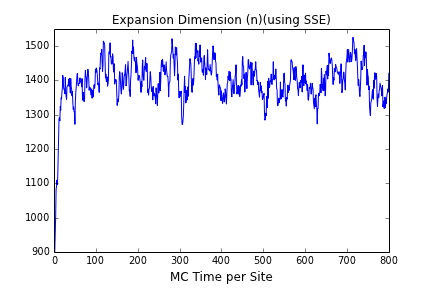
\includegraphics[width=100mm]
{../programs/graphics/metropolis_sse/n_T2,000000L32.png}
\caption{Equilibration of expansion dimension}
\end{figure}
\newpage
Then, look at equilibration time of states of spins:

\begin{figure}[ht]
\centering
\begin{minipage}[b]{0.45\linewidth}
\includegraphics[width=80mm]
{../programs/graphics/metropolis_sse/magnet_allup_T2,000000_L32.png}
\end{minipage}
\quad
\begin{minipage}[b]{0.45\linewidth}
\includegraphics[width=80mm]
{../programs/graphics/equilibration_time/magnet_allup_T2,000000_L32.png}
\caption{Equilibration of states via Metropolis algorithm with SSE and via 
Metropolis algorithm}
\end{minipage}
\end{figure}
\newpage

Also, we can look at autocorrelation function and correlation times,

\begin{figure}[ht]
\centering
\begin{minipage}[b]{0.45\linewidth}
\includegraphics[width=80mm]
{../programs/graphics/metropolis_sse/autocorrelation_T2,000000_L32.png}
\end{minipage}
\quad
\begin{minipage}[b]{0.45\linewidth}
\includegraphics[width=80mm]
{../programs/graphics/autocorrelation/autocorrelation_T2,000000_L32.png}
\caption{Autocorrelation function for magnetization via Metropolis 
algorithm with SSE and via Metropolis algorithm}
\end{minipage}
\end{figure}

\begin{figure}[ht]
\centering
\begin{minipage}[b]{0.45\linewidth}
\includegraphics[width=80mm]
{../programs/graphics/metropolis_sse/autocorrelation1_T2,000000_L32.png}
\end{minipage}
\quad
\begin{minipage}[b]{0.45\linewidth}
\includegraphics[width=80mm]
{../programs/graphics/autocorrelation/autocorrelation1_T2,000000_L32.png}
\caption{Early times of autocorrelation function for magnetization via 
Metropolis algorithm with SSE and via Metropolis algorithm}
\end{minipage}
\end{figure}


\begin{figure}[ht]
\centering
\begin{minipage}[b]{0.45\linewidth}
\includegraphics[width=80mm]
{../programs/graphics/metropolis_sse/correlation_fit_T2,000000_L32.png}
\end{minipage}
\quad
\begin{minipage}[b]{0.45\linewidth}
\includegraphics[width=80mm]
{../programs/graphics/autocorrelation/correlation_fit_T2,000000_L32.png}
\caption{Linear fitting to find correlation time for magnetization via 
Metropolis algorithm with SSE and via Metropolis algorithm}
\end{minipage}
\end{figure}

\newpage

So, expectations of properties at T=2.0 and L=32 are:

\begin{center}
    \begin{tabular}{ | l | l | p{5cm} |}
    \hline
    Property  & Metropolis with SSE & Metropolis \\ \hline
    Magnetization &  $(9.1151 \pm 0.0087) e-01$ & $(9.1039 \pm 
    0.0093)e-01$  \\ \hline
    Energy & $(-1.7456 \pm 0.0017) e+00$  & $(-1.7447 \pm 0.0018) 
    e+00$   \\ \hline
    Magnetic Susceptibility & $(3.882 \pm 0.239) e-01$ & $(4.463 \pm 
    0.306) e-01$   \\ \hline
    Specific Heat &$(7.4486 \pm 0.3431) e-01$ & $(8.0022 \pm 
    0.3687)e-01$ \\
    \hline
    \end{tabular}
\end{center}
(Errors are calculated with Jackknife method.)








Let's look at equilibration times when T=3.0 and L=32:
First, look at equilibration time of expansion dimension,n;
\begin{figure}[ht!]
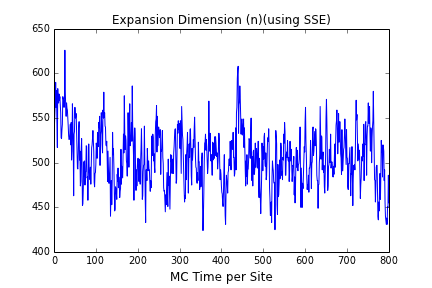
\includegraphics[width=100mm]
{../programs/graphics/metropolis_sse/n_T3,000000L32.png}
\caption{Equilibration of expansion dimension}
\end{figure}
\newpage
Then, look at equilibration time of states of spins:

\begin{figure}[ht]
\centering
\begin{minipage}[b]{0.45\linewidth}
\includegraphics[width=80mm]
{../programs/graphics/metropolis_sse/magnet_allup_T3,000000_L32.png}
\end{minipage}
\quad
\begin{minipage}[b]{0.45\linewidth}
\includegraphics[width=80mm]
{../programs/graphics/equilibration_time/magnet_allup_T3,000000_L32.png}
\caption{Equilibration of states via Metropolis algorithm with SSE and via 
Metropolis algorithm}
\end{minipage}
\end{figure}


\newpage
Also, we can look at autocorrelation function and correlation times,

\begin{figure}[ht]
\centering
\begin{minipage}[b]{0.45\linewidth}
\includegraphics[width=80mm]
{../programs/graphics/metropolis_sse/autocorrelation_T3,000000_L32.png}
\end{minipage}
\quad
\begin{minipage}[b]{0.45\linewidth}
\includegraphics[width=80mm]
{../programs/graphics/autocorrelation/autocorrelation_T3,000000_L32.png}
\caption{Autocorrelation function for magnetization via Metropolis 
algorithm with SSE and via Metropolis algorithm}
\end{minipage}
\end{figure}

\begin{figure}[ht]
\centering
\begin{minipage}[b]{0.45\linewidth}
\includegraphics[width=80mm]
{../programs/graphics/metropolis_sse/autocorrelation1_T3,000000_L32.png}
\end{minipage}
\quad
\begin{minipage}[b]{0.45\linewidth}
\includegraphics[width=80mm]
{../programs/graphics/autocorrelation/autocorrelation1_T3,000000_L32.png}
\caption{Early times of autocorrelation function for magnetization via 
Metropolis algorithm with SSE and via Metropolis algorithm}
\end{minipage}
\end{figure}


\begin{figure}[ht]
\centering
\begin{minipage}[b]{0.45\linewidth}
\includegraphics[width=80mm]
{../programs/graphics/metropolis_sse/correlation_fit_T3,000000_L32.png}
\end{minipage}
\quad
\begin{minipage}[b]{0.45\linewidth}
\includegraphics[width=80mm]
{../programs/graphics/autocorrelation/correlation_fit_T3,000000_L32.png}
\caption{Linear fitting to find correlation time for magnetization via 
Metropolis algorithm with SSE and via Metropolis algorithm}
\end{minipage}
\end{figure}

\newpage

 
So, expectations of properties at T=3.0 and L=32 are:

\begin{center}
    \begin{tabular}{ | l | l | p{5cm} |}
    \hline
    Property  & Metropolis with SSE & Metropolis \\ \hline
    Magnetization &  $(0.523 \pm 1.266) e-03 $ & $ (-2.427 \pm 
    1.274)e-03$  \\ \hline
    Energy & $(-8.182 \pm 0.007) e-01$  & $(-8.174 \pm 
    0.007)e-01 $   \\ \hline
    Magnetic Susceptibility & $(3.828 \pm 0.083) e+00 $ & $(3.876 
    \pm 0.064)e+00$   \\ \hline
    Specific Heat &$(3.970 \pm 0.087) e-01$ & $(4.027 \pm 0.070) e-01 
    $ \\
    \hline
    \end{tabular}
\end{center} 
(Errors are calculated with Jackknife method.)


%\chapter{Conclusion and Discussion}

\bibliography{kaplan_ifp_report}
\bibliographystyle{ieeetr}

\appendix
\chapter{Programs}
Here is the programs written in Python to simulate 2D Ising Model with 
Metropolis Algorithm, Metropolis Algorithm with SSE and Wolff Algorithm.
\lstset{
	language=Python,
	keywordstyle=\bfseries\ttfamily\color[rgb]{0,0,1},
	identifierstyle=\ttfamily,
	commentstyle=\color[rgb]{0.133,0.545,0.133},
	stringstyle=\ttfamily\color[rgb]{0.627,0.126,0.941},
	showstringspaces=false,
	basicstyle=\footnotesize,
	numberstyle=\footnotesize,
	numbers=left,
	stepnumber=2,
	numbersep=10pt,
	tabsize=2,
	breaklines=true,
	prebreak = \raisebox{0ex}[0ex][0ex]{\ensuremath{\hookleftarrow}},
	breakatwhitespace=false,
	aboveskip={1.5\baselineskip},
  columns=fixed,
  upquote=true,
  extendedchars=true,
 frame=lines,
}

\lstinputlisting[caption=Metropolis Algorithm]
{../programs/metropolis_report.py}

\lstinputlisting[caption=Metropolis Algorithm with SSE]
{../programs/metropolis_sse_report.py}

\lstinputlisting[caption=Wolff Algorithm]{../programs/wolff_report.py}


\end{document}




 





